\documentclass[11pt,a4paper]{article}
\usepackage[utf8]{inputenc}
\usepackage[margin=1in]{geometry}
\usepackage{amsmath,amssymb,amsfonts,amsthm}
\usepackage{booktabs}
\usepackage{graphicx}
\usepackage{natbib}
\usepackage{hyperref}
\usepackage{subcaption}
\usepackage{enumitem}
\usepackage{microtype}
\emergencystretch=3em
\usepackage{ctex}

\newtheorem{theorem}{定理}
\newtheorem{proposition}{命题}
\newtheorem{lemma}{引理}
\newtheorem{definition}{定义}
\newtheorem{remark}{注记}

\hypersetup{
    colorlinks=true,
    linkcolor=blue,
    citecolor=blue,
    urlcolor=blue,
    pdftitle={病例规模不再是主要推断瓶颈的边界：估计目标、监测杠杆与流感住院实证},
    pdfauthor={匿名评审稿}
}

\title{\textbf{\zihao{3} 病例规模不再是主要推断瓶颈的边界：\\估计目标、监测杠杆与流感住院实证}}
\author{\large （匿名评审稿）}
\date{\today}

\begin{document}

\maketitle

\begin{abstract}
\noindent 准确识别疫情增长并预测短期病例负担是传染病预警的核心任务。直观上病例数越多测量精度越高，但在个体超传播、监测漏报与周际环境扰动并存时，“样本量”与“信息量”不能简单等同。既有信息下界的标度律建立在当期再生数 $R_t$ 一类估计目标上；本文证明更换估计目标后标度律随之改变，据此将“病例规模何时不再是主要推断瓶颈”作为监测设计问题严格推导。主要结果：（i）在已知风险集 $n$、报告率 $\rho$ 与离散参数 $k$ 的负二项分支--二项报告基准模型下，矩估计量 $\widehat{R}_t = C_t/(\rho n)$ 为条件 MLE，方差达到 Fisher 信息逆，随 $m = \rho n$ 单调收敛于零；（ii）以该估计量推断跨期基础水平 $\bar{R}$ 时，方差受环境底板 $v_R$ 制约，由此导出环境项与规模项相等的平滑交叉点 $m_\times$；（iii）提高 $\rho$ 仅消除漏报抽稀方差，唯有扩大基数 $n$ 使各项方差同时衰减，预算约束下拉长观测期数以 $O(1/T)$ 削减环境方差；（iv）给出负二项单调似然比的精确增长判定检验与离散功效，并剥离事后增长统计量与事前单步预测的代数关系。实证方面，利用 CDC NHSN 2020--2026 年 16,218 个州周流感住院数据：仿射 FGLS 拟合得规模相关方差项 $b = 2.2434$（95\% CI $[1.50, 3.02]$）、与规模无关的经验损失截距 $a = 0.0991$、经验交叉点 22.6 例/周（对极端损失的处理敏感：截尾 1\% 后移至 10.6，属量级估计）；误差预算分解将平均误差定量为仿射拟合中与规模无关份额 54.6\%、规模项份额 45.1\%，样本中已实现的大规模观测（$D_t \ge 250$）误差约为全体平均的六成；达峰期总体误差约 89\% 来自平稳基准的常数偏差（各规模箱占比 59.5\%--94.8\% 不等）；统一损失尺度后达峰期内部规模项仍显著为正（$b=7.93$），其点估计低于初期（共同分母口径 1.85 对 2.24），但阶段差异未达统计显著（交互项 95\% CI 含零）——失效的是平稳性假定而非病例规模；时变交叉点在流感季（中位数 19.7--20.4）与非流感季（46.9--47.9）间系统性分离。上述量化参照为监测资源在规模与协变量之间的配置比较提供了量级判断。

\vspace{0.8em}
\noindent \textbf{关键词：} 疫情增长判定；分支过程；超传播；漏报；环境随机性；监测设计；短期预测；预测误差分解；流感住院实证
\end{abstract}

\vspace{1em}
\begin{center}
\textbf{\large The Boundary beyond Which Case Counts Are No Longer the Main \\
Inference Bottleneck: Estimation Targets, Monitoring Levers, and Influenza Hospitalization Evidence}
\end{center}

\vspace{1.5em}

\section{引言}\label{sec:intro}

准确识别疫情由下降转为增长，并对随后数周的病例负担作出前瞻预测，是传染病预警与应急响应的核心任务。直观上，病例数越多，随机计数波动的相对影响越小；但这一直观判断并不足以说明：在流行病学监测系统中，病例规模增加到什么程度后，增长判定或短期预测精度的改善会明显放缓？尤其当病原体传播具有高度个体异质性（超传播）、监测系统存在显著漏报、且同一时期内的感染者共同受到气象、人群接触模式等周际环境随机扰动时，“样本量”与“信息量”不再能够简单等同 \citep{lloydsmith2005superspreading, cori2013new}。

关于疫情监测数据中信息限制的研究已取得诸多奠基性成果。个体传播异质性的开创性工作表明，传统基于平均传播水平的推断严重掩盖了子代感染数的高度过离散 \citep{lloydsmith2005superspreading}；基于发病序列更新过程估计时变再生数的模型，则确立了现代实时监测的实用基准 \citep{cori2013new}。近年来，学者们进一步利用 Fisher 信息量框架系统探讨了不完全观测、报告延迟以及噪声疫情曲线所蕴含的信息损失 \citep{parag2022quantifying}，揭示了从实时再生数推断疫情反弹所面临的固有信息下界与非对称干预延迟 \citep{parag2022fundamental, parag2025asymmetric}。这些工作所刻画的下界，其信息量随期望病例数增长的标度律是在\textbf{当期再生数} $R_t$ 一类的估计目标下建立的。本文与之形成正面对话：\textbf{下界的标度律在更换估计目标后随之改变}——对当期 $R_t$，规模的边际方差收益恒为正（命题~\ref{prop:measurement_var}）；对跨期基础水平 $\bar{R}$，规模的边际收益在环境方差底板处放缓并受交叉点 $m_\times$ 标定（命题~\ref{prop:trend_var}）。换言之，"病例数是不是瓶颈"不是问题的属性，而是\textbf{估计目标的属性}，这一目标依赖性为既有信息下界框架补充了一个此前未显式刻画的维度。在统计推断层面，针对存在系统性漏报的疾病监测序列，状态空间与序列更新模型也已得到系统发展，强调了潜在未观测感染压力与已报告序列之间的状态剥离 \citep{bracher2021marginal, bhatt2023semi, steyn2025primer}。此外，人口统计随机性与共同环境随机性的区分在非线性流行病学模型中亦具有悠久的理论渊源 \citep{rasmussen2011inference, aber2025timeseries}。

然而，对“病例规模何时不再是主要推断瓶颈”的回答，首先取决于\textbf{究竟要估计什么}。如果推断目标是当期环境条件下的特定传播参数，那么在模型正确设定的理想条件下，更多病例可以不断提高对该参数的测量精度；但如果目标是跨周稳定的潜在基础增长趋势，则单周病例数即使非常巨大，在缺乏外部环境协变量时，也无法仅凭这一周的数据消除共同环境扰动。类似地，在固定报告率下已知真实感染风险集、仅有报告病例作为分母、以及报告率本身随时间变化，是三个完全不同的观测问题，绝不能将同一个样本量公式无条件推广。

本文的贡献\textbf{不在于单独提出新的负二项分支模型或漏报校正公式，也不在于宣称发现了某种不可逾越的通用信息论硬极限}。本文的差异化定位在于：针对“病例规模何时不再主导推断误差”这一具体监测设计问题，建立一个分层随机推断框架：
\begin{enumerate}[label=(\arabic*)]
\item \textbf{明确估计目标与饱和范畴}：严格区分\textbf{当期环境条件下的传播参数 $R_t$} 与\textbf{跨期基础水平 $\bar{R}$}，证明二者对增加病例规模的边际方差响应截然不同，并解析导出单期指定估计量方差内部环境项与抽样项相等的平滑交叉点 $m_\times$。
\item \textbf{精确拆解监测杠杆的非对称性}：证明“扩大真实感染基数 $n$（人群/地理覆盖扩大）”与“提高检测报告率 $\rho$”存在数理非对称性——显式分解指出提高报告率仅能消除漏报抽稀方差 $\frac{(1-\rho)\bar{R}}{\rho n}$，无法消除完全报告时依然存在的计数方差与超传播内在抽样方差；唯有扩大真实基数才能使两项方差同时衰减。
\item \textbf{分析理想设计下的监测维度权衡}：在理想化重复采样设计与总期望捕获病例预算 $B = T \cdot m$ 约束下，严格推导拉长独立观测期数 $T$ 削减环境方差 $v_R$ 的精确表达式，并明确指出每期整数风险集约束下的离散可行设计集合。
\item \textbf{给出增长判定检验与预测基准评估}：导出基于负二项离散尾概率的精确上尾超临界增长判定检验；在时间序列更新过程中清晰界定事后代理增长统计量与事前单步病例预测的内在代数关系与条件方差展开，并通过有限样本模拟检验理论基准的适用性与衰减形态。
\item \textbf{真实监测数据实证与误差预算分解：}采用美国疾控中心国家医疗保健安全网（CDC NHSN）2020--2026 年覆盖 50 个州及华盛顿特区周度流感住院真实数据（16,218 个州周观测），在控制聚类不确定性的前提下，测得经验收益放缓平台的数量级与报告政策切换前后的离散度分化，识别出达峰期失效的是跨期平稳基准假定而非病例规模本身，并给出\textbf{误差预算份额分解}与\textbf{时变经验交叉点}：过半误差份额落在与规模无关的拟合项上，样本中已实现的大规模观测误差约为全体平均的六成——过半误差与规模无关这一结构本身，提示进一步评估环境协变量与多期信息的价值。
\end{enumerate}

\section{模型与估计目标}\label{sec:methods}

\subsection{传播与报告模型}\label{subsec:meth_model}

设上一传播代有 $n$ 名真实感染者，第 $i$ 名感染者产生的继发感染数为 $X_{i,t}$。在给定当期环境条件下的传播参数 $R_t$ 后，假设个体继发感染数服从过离散负二项分支分布：
\begin{equation}
\mathbb{E}[X_{i,t} \mid R_t] = R_t, \qquad
\operatorname{Var}(X_{i,t} \mid R_t) = R_t + \frac{R_t^2}{k}, \label{eq:nb_branching}
\end{equation}
其中 $k > 0$ 为个体传播离散参数（$k \to 0$ 对应极端超传播，$k \to \infty$ 退化为泊松分布）。假设在给定 $(n, R_t)$ 条件下，个体继发感染数 $\{X_{i,t}\}_{i=1}^n$ 相互条件独立。当期真实新发感染总数为 $I_t = \sum_{i=1}^n X_{i,t}$。

观测过程采用固定报告率 $\rho \in (0, 1]$ 的基准二项抽稀模型：
\begin{equation}
C_t \mid I_t \sim \operatorname{Binomial}(I_t, \rho). \label{eq:binomial_obs}
\end{equation}
\textbf{理论基准设定}：第~\ref{sec:theory} 节的推导在\textbf{已知真实风险集规模 $n$} 的条件下建立理论基准，使各类方差分量的机制来源获得解析透明的对照参照系；第~\ref{subsec:theory_multistep} 节进一步给出仅报告数据可见时的条件预测方差分解，并说明单代基准不能直接移用。

\subsection{两种不同的估计目标}\label{subsec:meth_targets}

在推导方差前，必须严格区分两类性质迥异的估计目标：
\begin{itemize}
\item \textbf{目标 A（当期传播参数）：} 估计给定当期环境条件下的传播参数 $R_t$。目标是测量当期环境（包含当周气象、人群接触模式等共同扰动）所决定的个体期望继发感染水平。注意：该参数不同于最终实现的感染比例 $I_t/n$，后者还叠加了个体分支过程的抽样随机性。
\item \textbf{目标 B（跨期基础水平）：} 估计消除单周共同随机扰动后的潜在基础增长趋势 $\bar{R}$。
\end{itemize}
在单期基准设计中，给定风险集规模 $n$ 后，假定当期环境满足条件矩设定：
\begin{equation}
\mathbb{E}[R_t \mid n] = \bar{R}, \qquad \operatorname{Var}(R_t \mid n) = v_R > 0. \label{eq:env_conditional_moment}
\end{equation}
这一条件可由固定试验设计的 $n$，或 $R_t$ 与 $n$ 相互独立作为充分条件予以保证。

\subsection{预测信息集}\label{subsec:meth_infoset}

针对预测问题，其表现依赖于当前可用的信息集。本文严格区分两种信息集：
\begin{itemize}
\item \textbf{全历史信息集 $\mathcal{F}_t^I$：} $\mathcal{F}_t^I = \sigma(I_1, \dots, I_t, C_1, \dots, C_t)$。在此理想信息集下，截至第 $t$ 期的历史真实感染完全可知，未来的感染压力 $\Lambda_{t+1}$ 是已确定的历史量。
\item \textbf{仅报告序列信息集 $\mathcal{F}_t^C$：} $\mathcal{F}_t^C = \sigma(C_1, C_2, \dots, C_t)$。这是现实监测中唯一可直接获取的信息，满足 $\mathcal{F}_t^C \subset \mathcal{F}_t^I$。由于二项漏报的存在，$I_1, \dots, I_t$ 未被完全观测，下一周的潜在感染压力 $\Lambda_{t+1}$ 本身具有不确定性，成为随机变量。
\end{itemize}

\section{理论结果}\label{sec:theory}

\subsection{当期传播参数、Fisher 信息与条件方差}\label{subsec:theory_var}

\begin{proposition}[\textbf{当期传播参数的条件似然、Fisher 信息与方差}]\label{prop:measurement_var}
在个体继发感染条件独立且服从负二项模型~\eqref{eq:nb_branching}、二项报告率 $\rho$ 固定的基准条件下，当真实风险集 $n$ 与报告率 $\rho$ 已知时：
\begin{enumerate}[label=(\roman*)]
\item 报告病例数 $C_t$ 在给定 $(n, R_t)$ 下的边缘分布严格服从负二项分布：
\begin{equation}
C_t \mid n, R_t \sim \operatorname{NB}\!\left(\text{均值} = \rho n R_t, \; \text{形状参数} = nk\right); \label{eq:nb_thinning}
\end{equation}
\item 矩估计量 $\widehat{R}_t = \frac{C_t}{\rho n}$ 恰为该条件似然模型下 $R_t$ 的极大似然估计量（MLE）；当观测值 $C_t = 0$ 时，$\widehat{R}_t = 0$ 位于非负参数空间的边界；
\item 在内部参数点 $R_t \in (0, \infty)$ 上，该模型关于 $R_t$ 的 Fisher 信息量为：
\begin{equation}
\mathcal{I}(R_t \mid n) = \frac{n}{\frac{R_t}{\rho} + \frac{R_t^2}{k}}; \label{eq:fisher_info}
\end{equation}
\item 估计量 $\widehat{R}_t$ 的条件方差严格达到 Cramér--Rao 下界：
\begin{equation}
\operatorname{Var}\!\left(\frac{C_t}{\rho n} \;\middle|\; n, R_t\right) = \mathcal{I}(R_t \mid n)^{-1} = \frac{R_t}{\rho n} + \frac{R_t^2}{k n}. \label{eq:var_prop1}
\end{equation}
\end{enumerate}
\end{proposition}

\begin{proof}
由负二项分布的概率生成函数（PGF），若个体继发感染数 $X_{i,t} \sim \operatorname{NB}(k, p)$，其中 $p = \frac{k}{k + R_t}$，则 $I_t = \sum_{i=1}^n X_{i,t} \sim \operatorname{NB}(nk, p)$，其 PGF 为 $G_{I_t}(s) = \left(\frac{p}{1 - (1-p)s}\right)^{nk}$。
在二项抽样 $C_t \mid I_t \sim \operatorname{Binomial}(I_t, \rho)$ 下，复合分布的 PGF 为：
\begin{equation*}
G_{C_t}(s) = G_{I_t}(1 - \rho + \rho s) = \left(\frac{p}{1 - (1-p)(1 - \rho + \rho s)}\right)^{nk} = \left(\frac{p^*}{1 - (1-p^*)s}\right)^{nk},
\end{equation*}
其中 $p^* = \frac{p}{p + \rho(1-p)} = \frac{k}{k + \rho R_t}$。这证明了 $C_t \mid n, R_t$ 服从形状参数为 $nk$、成功概率为 $p^*$ 的负二项分布，条件均值为 $\rho n R_t$。

其对数似然函数为：
\begin{equation*}
\ln L(R_t) = \text{const} - (nk + C_t) \ln(k + \rho R_t) + C_t \ln R_t.
\end{equation*}
对 $R_t$ 求导并令得分为零：
\begin{equation*}
\frac{\partial \ln L}{\partial R_t} = -\frac{\rho(nk + C_t)}{k + \rho R_t} + \frac{C_t}{R_t} = \frac{k(C_t - \rho n R_t)}{R_t(k + \rho R_t)} = 0 \implies \widehat{R}_t^{\text{MLE}} = \frac{C_t}{\rho n}.
\end{equation*}
计算得分函数的方差以求 Fisher 信息量：
\begin{equation*}
\mathcal{I}(R_t \mid n) = \operatorname{Var}\left(\frac{\partial \ln L}{\partial R_t}\right) = \frac{k^2 \operatorname{Var}(C_t \mid n, R_t)}{R_t^2(k + \rho R_t)^2}.
\end{equation*}
代入负二项方差 $\operatorname{Var}(C_t \mid n, R_t) = \rho n R_t + \frac{\rho^2 n R_t^2}{k} = \frac{\rho n R_t(k + \rho R_t)}{k}$：
\begin{equation*}
\mathcal{I}(R_t \mid n) = \frac{k^2 \cdot \frac{\rho n R_t(k + \rho R_t)}{k}}{R_t^2(k + \rho R_t)^2} = \frac{k \rho n R_t}{R_t^2(k + \rho R_t)} = \frac{n}{\frac{R_t}{\rho} + \frac{R_t^2}{k}}.
\end{equation*}
因此其倒数恰为 $\operatorname{Var}(\widehat{R}_t \mid n, R_t) = \frac{R_t}{\rho n} + \frac{R_t^2}{kn}$。
\end{proof}

\begin{remark}[\textbf{边界限定}]
命题~\ref{prop:measurement_var} 清晰建立了病例数所携带的 Fisher 信息量 $\mathcal{I}(R_t \mid n) \propto n$ 与方差的关系。但必须明确：这是\textbf{在已知真实风险集 $n$、已知报告率 $\rho$、模型正确设定且估计当期传播参数 $R_t$} 的条件结果，不能直接搬到仅能观测报告序列或估计跨期基础水平 $\bar{R}$ 的问题中。
\end{remark}

\subsection{跨期基础水平的单期边际方差}\label{subsec:theory_trend}

\begin{proposition}[\textbf{跨期基础水平的单期边际方差}]\label{prop:trend_var}
在条件矩假设~\eqref{eq:env_conditional_moment} 下，若使用单期估计量 $\frac{C_t}{\rho n}$ 估计跨期基础水平 $\bar{R}$，其给定风险集 $n$ 的条件边际方差为：
\begin{equation}
\operatorname{Var}\!\left(\frac{C_t}{\rho n} \;\middle|\; n\right) = v_R + \frac{\bar{R}}{\rho n} + \frac{\bar{R}^2 + v_R}{k n}. \label{eq:var_prop2}
\end{equation}
\end{proposition}

\begin{proof}
应用全方差公式以 $\bar{R}$ 为目标分解：
\begin{equation*}
\operatorname{Var}\!\left(\frac{C_t}{\rho n} \;\middle|\; n\right) = \operatorname{Var}\left(\mathbb{E}\left[\frac{C_t}{\rho n} \;\middle|\; n, R_t\right] \;\middle|\; n\right) + \mathbb{E}\left[\operatorname{Var}\left(\frac{C_t}{\rho n} \;\middle|\; n, R_t\right) \;\middle|\; n\right].
\end{equation*}
由命题~\ref{prop:measurement_var}，第一项为 $\operatorname{Var}(R_t \mid n) = v_R$。第二项为：
\begin{equation*}
\mathbb{E}\left[\frac{R_t}{\rho n} + \frac{R_t^2}{k n} \;\middle|\; n\right] = \frac{\mathbb{E}[R_t \mid n]}{\rho n} + \frac{\mathbb{E}[R_t^2 \mid n]}{k n}.
\end{equation*}
利用条件二阶矩关系 $\mathbb{E}[R_t^2 \mid n] = \operatorname{Var}(R_t \mid n) + (\mathbb{E}[R_t \mid n])^2 = v_R + \bar{R}^2$，相加即得式~\eqref{eq:var_prop2}。
\end{proof}

\begin{remark}[\textbf{单期设计的方差底板限定}]
式~\eqref{eq:var_prop2} 中的 $v_R$ 底板，是在\textbf{指定单期估计量 $\widehat{R}_t = C_t/(\rho n)$、无外部协变量、且仅依据单期数据}推断跨期基础水平 $\bar{R}$ 的严格条件方差下界。这并不排斥通过引入气象/人群接触等显式环境协变量、采用多期时间序列状态平滑或贝叶斯动态滤波来进一步降低后验方差；它界定的是仅凭单期病例聚合本身所无法消除的共同随机性部分。
\end{remark}

\subsection{方差占比交叉点 $m_\times$}\label{subsec:theory_crossover}

令 $m = \rho n$ 为\textbf{上一代真实风险集对应的期望被报告人数}（当期新发报告数的条件期望为 $\rho n R_t$，两者在 $R_t$ 波动下不等；图注与政策讨论中的“期望报告病例数”均取本定义）。式~\eqref{eq:var_prop2} 可重写为 $v_R + A/m$，其中
\begin{equation}
A = \bar{R} + \frac{\rho(\bar{R}^2 + v_R)}{k}.
\end{equation}
我们称 $A/m$ 为\textbf{病例规模相关方差项}。

\begin{definition}[\textbf{方差占比交叉点}]\label{def:crossover}
当 $v_R > 0$ 时，在基础水平单期估计方差式~\eqref{eq:var_prop2} 内部，病例规模相关方差项 $A/m$ 与共同环境方差项 $v_R$ 相等的期望报告病例规模定义为方差占比交叉点：
\begin{equation}
m_\times \triangleq \frac{A}{v_R} = \frac{\bar{R} + \rho(\bar{R}^2 + v_R)/k}{v_R}. \label{eq:crossover_def}
\end{equation}
\end{definition}

\paragraph{经济学与监测含义：} $m_\times$ 的解释是“在给定 $(\rho, k, \bar{R}, v_R)$ 下，沿扩大 $n$ 方向时两类方差相等的规模”。在 $m = m_\times$ 处，总方差中两项各占 50\%。导数 $\frac{\mathrm{d}V}{\mathrm{d}m} = -\frac{A}{m^2}$ 在 $m_\times$ 处平滑连续，不存在突变。当 $m > m_\times$ 时，环境方差占主导，增加病例数仍能降低方差，但仅能作用于占比逐渐减小的 $A/m$ 项。

\begin{figure}[htbp]
\centering
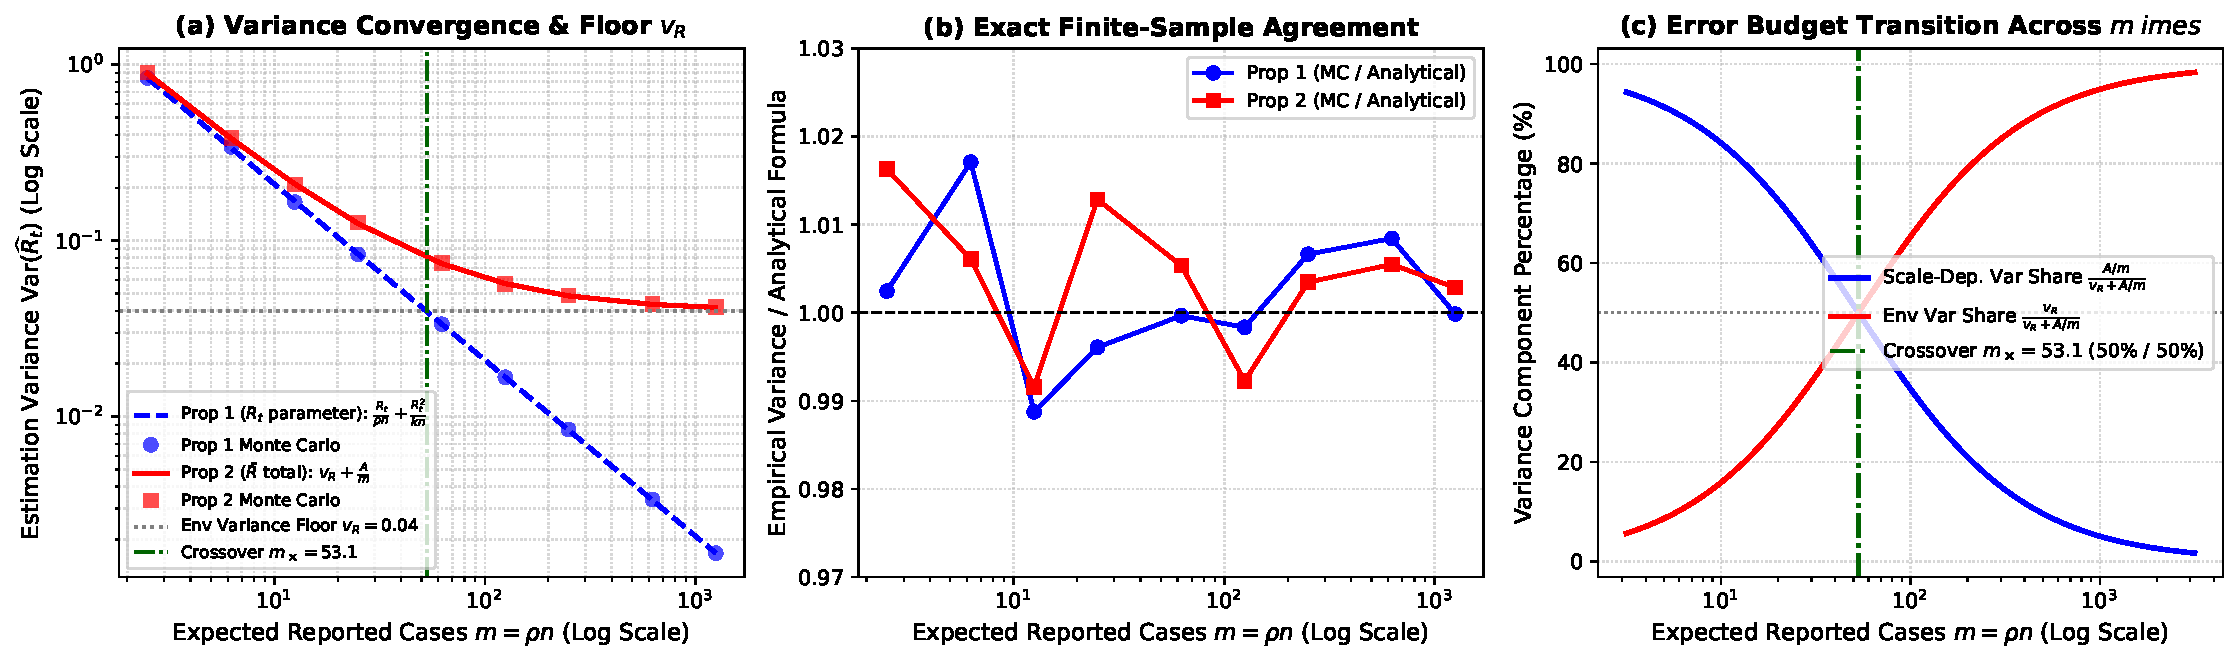
\includegraphics[width=\textwidth]{../figures/fig1_theory_simulation_verification.pdf}
\caption{\textbf{理论命题与方差占比交叉点蒙特卡洛验证}（50,000 次模拟，参数设定 $\bar{R}=1.15, v_R=0.04, k=0.35, \rho=0.25$）。(a) 当期传播参数测量方差式~\eqref{eq:var_prop1}（蓝）与跨期基础水平单期方差式~\eqref{eq:var_prop2}（红）随期望报告病例数 $m = \rho n$ 的双对数衰减曲线，数值模拟散点与理论解析曲线一致，清楚展现环境方差底板 $v_R = 0.04$；(b) 经验方差与理论推导公式的比值在本次参数网格下处于 0.988--1.017 之间，有限样本模拟值接近解析值；(c) 误差预算动态演变：在交叉点 $m_\times = 53.1$ 处，病例规模相关方差与环境扰动各占 50\%，展现了主要误差来源的平滑交接。}
\label{fig:theory_verification}
\end{figure}

\subsection{监测杠杆的非对称性：样本基数 $n$ 与报告率 $\rho$ 的精确拆解}\label{subsec:theory_levers}

在公共卫生监测实践中，增加报告病例数 $m = \rho n$ 存在两条截然不同的政策路径：其一是\textbf{扩大监测捕获基数 $n$}（如扩大哨点覆盖范围、汇总跨区域感染者）；其二是\textbf{提高报告率 $\rho$}（如加强密切接触者筛查、降低就医检测门槛）。我们将式~\eqref{eq:var_prop2} 明确拆解为关于 $(n, \rho)$ 的二元函数：
\begin{equation}
V(n, \rho) = v_R + \frac{\bar{R}}{\rho n} + \frac{\bar{R}^2 + v_R}{k n}. \label{eq:var_bivariate}
\end{equation}
为彻底理清报告率 $\rho$ 的作用机制，我们将第二项恒等拆解为：
\begin{equation}
\frac{\bar{R}}{\rho n} = \underbrace{\frac{\bar{R}}{n}}_{\text{完全报告时仍有的计数波动}} + \underbrace{\frac{(1-\rho)\bar{R}}{\rho n}}_{\text{漏报额外引入的抽稀方差}}. \label{eq:rho_decomp}
\end{equation}

\begin{proposition}[\textbf{监测杠杆的非对称性与超传播方差下界}]\label{prop:levers_asymmetry}
在单期观测设计下，扩大基数 $n$ 与提高报告率 $\rho$ 对估计方差的削减效应存在本质非对称性：
\begin{enumerate}[label=(\roman*)]
\item \textbf{报告率杠杆的饱和下界：} 给定任意有限风险集规模 $n < \infty$，当报告率趋于理想极限（$\rho \to 1$，即完全无漏报监测）时，漏报额外抽稀方差项 $\frac{(1-\rho)\bar{R}}{\rho n} \to 0$，但估计方差存在严格大于环境底板的固有下界：
\begin{equation}
\lim_{\rho \to 1} V(n, \rho) = v_R + \frac{\bar{R}}{n} + \frac{\bar{R}^2 + v_R}{k n} > v_R. \label{eq:rho_limit}
\end{equation}
提高报告率消除的是漏报额外引入的抽稀方差，\textbf{无法消除完全报告时依然存在的计数波动 $\frac{\bar{R}}{n}$，更无法消除由个体超传播（$k$）引起的内在子代抽样随机性 $\frac{\bar{R}^2+v_R}{kn}$}；
\item \textbf{样本基数杠杆的全域收敛性：} 无论报告率 $\rho \in (0, 1]$ 处于何种水平，只要扩大真实风险集规模至极限（$n \to \infty$），两项病例规模相关方差均严格收敛于零：
\begin{equation}
\lim_{n \to \infty} V(n, \rho) = v_R.
\end{equation}
\end{enumerate}
\end{proposition}

\begin{proof}
将式~\eqref{eq:rho_decomp} 代入式~\eqref{eq:var_bivariate} 分别令 $\rho \to 1$ 与 $n \to \infty$，代入极限直接即得。
\end{proof}

\begin{remark}[\textbf{公共卫生监测资源配置启示与适用边界}]\label{rem:levers}
命题~\ref{prop:levers_asymmetry} 揭示了监测杠杆的数理不对称性：在小风险集且个体传播高度离散时，单纯提高报告率无法消除个体传播抽样波动。然而，\textbf{该数理极限并不直接等同于现实中的绝对政策配置排序}。在实际流行病学监测决策中，跨区域汇总扩大 $n$ 可能会引入不同地理区域间传播参数 $R_t$、超传播 $k$ 和环境扰动的空间异质性；同时，扩大哨点覆盖与提升就医检测率的边际实施成本与数据延迟各不相同。因此，决策者应将该命题作为理解噪声结构构成的理论参照，结合具体干预的可行性与成本展开综合评估。
\end{remark}

\subsection{理想设计下的监测维度权衡：单期规模 vs 跨期跨度}\label{subsec:theory_budget}

进一步探讨监测资源分配的理论边界。考虑如下\textbf{理想化重复采样设计}：设设计者在 $T$ 个观测期内设定相同的每期真实风险集规模 $n_T = B/(\rho T)$，记为设计方案 $D_T = (T, n_T)$；跨期基础水平 $\bar{R}$、报告率 $\rho$、个体离散参数 $k$ 与环境方差 $v_R$ 保持不变。给定完整环境扰动序列后，各期继发分支与报告抽样过程条件独立，且条件均值为零。

基于设计 $D_T$ 的 $T$ 期观测数据，估计跨期基础水平 $\bar{R}$ 的样本均值估计量定义为：
\begin{equation}
\overline{\widehat{R}}_T \triangleq \frac{1}{T} \sum_{t=1}^T \widehat{R}_t = \frac{1}{T} \sum_{t=1}^T \frac{C_t}{\rho n_T}.
\end{equation}

\begin{proposition}[\textbf{预算约束下的监测设计权衡与可行性集合}]\label{prop:budget_tradeoff}
在上述理想化重复采样设计下，若总监测输入规模（各期期望被报告风险集人数之和）受限为 $B = T \cdot m$（其中 $m = \rho n_T$ 为每期上一代风险集对应的期望被报告人数，见第~\ref{subsec:theory_crossover} 节）：
\begin{enumerate}[label=(\roman*)]
\item 若各期环境扰动跨期条件独立，在设计 $D_T$ 下平均估计量的方差为：
\begin{equation}
\operatorname{Var}(\overline{\widehat{R}}_T \mid n_T) = \frac{v_R}{T} + \frac{A}{B}, \label{eq:var_budget_indep}
\end{equation}
其中 $A = \bar{R} + \rho(\bar{R}^2 + v_R)/k$。当总预算 $B$ 固定时，比较不同设计 $D_T$，增加观测期数 $T$（相应减少每期样本 $m = B/T$）严格单调降低估计方差；
\item 若各期环境扰动存在一阶自回归自相关 $\operatorname{Cov}(R_t, R_{t+s} \mid n_T) = v_R r^{|s|}$（$0 \le r < 1$），则有限期数 $T$ 下的精确方差为：
\begin{equation}
\operatorname{Var}(\overline{\widehat{R}}_T \mid n_T) = \frac{v_R}{T}\left[\frac{1+r}{1-r} - \frac{2r(1-r^T)}{T(1-r)^2}\right] + \frac{A}{B}, \label{eq:var_budget_ar1}
\end{equation}
在大期数极限 $T \gg 1$ 下，其渐近形式可表示为有效独立期数近似：
\begin{equation}
\operatorname{Var}(\overline{\widehat{R}}_T \mid n_T) \approx \frac{v_R}{T_{\operatorname{eff}}(T, r)} + \frac{A}{B}, \qquad T_{\operatorname{eff}}(T, r) \triangleq T \frac{1-r}{1+r};
\end{equation}
\item \textbf{离散可行设计集合：} 当要求各期风险集相同且为正整数（$n_T \in \mathbb{N}_+$），并精确用尽总预算 $B$ 时，设计者仅能在如下离散可行集合中比较期数：
\begin{equation}
\mathcal{T}(B, \rho) \triangleq \left\{ T \in \mathbb{N}_+ \;:\; \frac{B}{\rho T} \in \mathbb{N}_+ \right\}. \label{eq:feasible_T}
\end{equation}
若 $B/\rho \in \mathbb{N}_+$，可行期数为其正整数因子集合；不等式 $T \le \lfloor B/\rho \rfloor$ 仅是属于该集合的必要条件而非充分条件。
\end{enumerate}
\end{proposition}

\begin{proof}
由全方差公式，由于给定环境序列后分支与抽样过程条件独立，平均估计量的方差严格分解为环境项与抽样项：
\begin{align*}
\operatorname{Var}(\overline{\widehat{R}}_T \mid n_T) &= \frac{1}{T^2}\operatorname{Var}\left(\sum_{t=1}^T R_t \;\middle|\; n_T\right) + \frac{1}{T^2}\sum_{t=1}^T \mathbb{E}\big[\operatorname{Var}(\widehat{R}_t \mid n_T, R_t) \;\big|\; n_T\big] \\
&= \frac{1}{T^2}\operatorname{Var}\left(\sum_{t=1}^T R_t \;\middle|\; n_T\right) + \frac{A}{T(\rho n_T)}.
\end{align*}
将 $n_T = B/(\rho T)$ 代入抽样项，即得 $\rho n_T = B/T$，从而第二项恒为 $A/B$。在环境跨期独立假定下，第一项化为 $v_R/T$，相加直接得式~\eqref{eq:var_budget_indep}。若各期环境扰动存在一阶自回归自相关，利用平稳协方差双重求和展开：
\begin{equation*}
\operatorname{Var}\left(\sum_{t=1}^T R_t \;\middle|\; n_T\right) = T v_R + 2 v_R \sum_{s=1}^{T-1} (T-s) r^s = v_R T \left[\frac{1+r}{1-r} - \frac{2r(1-r^T)}{T(1-r)^2}\right].
\end{equation*}
除以 $T^2$ 即得式~\eqref{eq:var_budget_ar1}。当 $T \gg 1$ 时忽略 $O(1/T^2)$ 项，直接得到有效期数近似。最后由 $n_T = B/(\rho T) \in \mathbb{N}_+$ 即得式~\eqref{eq:feasible_T}。
\end{proof}

\begin{remark}[\textbf{理论决策含义与真实传播限制}]
式~\eqref{eq:var_budget_indep} 表明：\textbf{在本文限定的固定总预算、单地区、无外部环境协变量的理想设计中}，病例规模相关方差项 $A/B$ 保持不变；唯有通过在可行集合 $\mathcal{T}(B, \rho)$ 内增加观测期数 $T$，方能以 $O(1/T)$ 削减共同环境随机性 $v_R$。需要强调的是，真实疫情的时间序列具有自回归传染卷积，感染风险集往往受上一期影响而无法由设计者任意自由拆分。因此，该命题给出的是理想设计对比下的数理边界。
\end{remark}

\subsection{当期超临界增长判定检验与离散检出功效}\label{subsec:theory_growth_test}

利用式~\eqref{eq:nb_thinning} 的精确负二项条件分布，可直接建立基准模型下判定当期超临界增长（$R_t > 1$）的统计检验。考虑单侧假设检验问题：
\begin{equation}
H_0: R_t \le 1 \qquad \text{对} \qquad H_1: R_t > 1. \label{eq:hypo_growth}
\end{equation}

\begin{proposition}[\textbf{当期超临界增长判定检验与精确离散功效}]\label{prop:growth_test}
在已知 $(n, \rho, k)$ 的基准模型下：
\begin{enumerate}[label=(\roman*)]
\item 负二项分布族关于充分统计量 $C_t$ 具有单调似然比（Monotone Likelihood Ratio, MLR）性质；采用拒绝域 $\{C_t \ge c_\alpha\}$ 的非随机化上尾检验，在复合原假设 $H_0: R_t \le 1$ 下将第一类错误率严格控制在 $\alpha$ 以内：由 MLR，尾部概率 $\Pr_{R_t}(C_t \ge c)$ 关于 $R_t$ 单调不减，故 $\sup_{R_t \le 1} \Pr_{R_t}(C_t \ge c_\alpha) = \Pr_{R_t = 1}(C_t \ge c_\alpha)$，即水平控制在边界点 $R_t = 1$ 处取上确界，只需在该点校准即可。离散临界值 $c_\alpha \in \mathbb{N}$ 取使边界处超额拒绝概率受控的最小整数：
\begin{equation}
c_\alpha = \min \left\{ c \in \mathbb{N} \;:\; \Pr_{R_t = 1}(C_t \ge c) \le \alpha \right\}; \label{eq:crit_val}
\end{equation}
\item 对于任意给定的备择增长强度 $R_t = 1 + \delta$（$\delta > 0$），该非随机化检验的理论检出功效由下式精确给出：
\begin{equation}
\pi(n, \delta) \triangleq \Pr_{R_t = 1 + \delta}(C_t \ge c_\alpha) = 1 - F_{\operatorname{NB}}\!\left(c_\alpha - 1; \; nk, \; \frac{k}{k + \rho(1+\delta)}\right), \label{eq:power_exact}
\end{equation}
其中 $F_{\operatorname{NB}}(x; r, p) = \sum_{j=0}^{\lfloor x \rfloor} \frac{\Gamma(j+r)}{j!\Gamma(r)} p^r (1-p)^j$ 为负二项累积分布函数。
\end{enumerate}
\end{proposition}

\begin{remark}[\textbf{检验性质与多期反弹识别的区别}]
由于报告计数的非负离散性，非随机化检验在大多数有限样本下实际水平 $\Pr_{R_t=1}(C_t \ge c_\alpha)$ 严格小于名义水平 $\alpha$（呈现保守性）。更重要的是，命题~\ref{prop:growth_test} 判定的是\textbf{当期单代传播参数是否超临界（$R_t > 1$）}。这与流行病学中基于多期时序轨迹的“疫情反弹实时识别（Resurgence Detection）”具有本质区别 \citep{parag2022fundamental}：后者需要推断系统状态由亚临界向超临界的跨期转变过程，而单期检验仅评估当期横截面信号的统计显著性。
\end{remark}

\subsection{预测误差的条件分解：仅报告数据可见时的严格形式}\label{subsec:theory_multistep}

在现实流行病学监测中，真实感染历史不可见，决策者仅能依据报告历史 $\mathcal{F}_t^C$ 进行前瞻推断。引入更新过程描述跨周感染压力：
\begin{equation}
\Lambda_{t+1} = \sum_{s=1}^S w_s I_{t+1-s}, \qquad \sum_{s=1}^S w_s = 1.
\end{equation}
假设在给定潜变量与报告历史下满足：
\begin{equation}
\mathbb{E}[I_{t+1} \mid \Lambda_{t+1}, R_{t+1}, \mathcal{F}_t^C] = \Lambda_{t+1} R_{t+1}.
\end{equation}
并且，在给定当期真实感染数 $I_{t+1}$ 条件下，报告抽样过程 $C_{t+1} \mid I_{t+1} \sim \operatorname{Binomial}(I_{t+1}, \rho)$ 条件独立于既往报告历史 $\mathcal{F}_t^C$。

\begin{proposition}[\textbf{真实感染与报告病例的单步预测方差分解}]\label{prop:forecast_decomp}
基于截至第 $t$ 期的报告信息集 $\mathcal{F}_t^C$，未来真实感染数 $I_{t+1}$ 的预测方差严格满足全方差恒等式：
\begin{equation}
\operatorname{Var}(I_{t+1} \mid \mathcal{F}_t^C) = \operatorname{Var}\big(\Lambda_{t+1} R_{t+1} \;\big|\; \mathcal{F}_t^C\big) + \mathbb{E}\Big[\operatorname{Var}\big(I_{t+1} \;\big|\; \Lambda_{t+1}, R_{t+1}, \mathcal{F}_t^C\big) \;\Big|\; \mathcal{F}_t^C\Big]. \label{eq:var_I_decomp}
\end{equation}
在上述二项观测假定下，未来报告病例数 $C_{t+1}$ 的预测方差严格由下式给出：
\begin{equation}
\operatorname{Var}(C_{t+1} \mid \mathcal{F}_t^C) = \rho(1 - \rho)\,\mathbb{E}[I_{t+1} \mid \mathcal{F}_t^C] + \rho^2 \operatorname{Var}(I_{t+1} \mid \mathcal{F}_t^C). \label{eq:var_C_decomp}
\end{equation}
\end{proposition}

\begin{proof}
对 $I_{t+1}$ 以 $(\Lambda_{t+1}, R_{t+1})$ 为条件应用全方差公式，即得式~\eqref{eq:var_I_decomp}。对于报告病例 $C_{t+1}$，以 $I_{t+1}$ 为条件应用全方差公式：
\begin{equation*}
\operatorname{Var}(C_{t+1} \mid \mathcal{F}_t^C) = \mathbb{E}[\operatorname{Var}(C_{t+1} \mid I_{t+1}, \mathcal{F}_t^C) \mid \mathcal{F}_t^C] + \operatorname{Var}(\mathbb{E}[C_{t+1} \mid I_{t+1}, \mathcal{F}_t^C] \mid \mathcal{F}_t^C).
\end{equation*}
由条件独立假定 $C_{t+1} \mid (I_{t+1}, \mathcal{F}_t^C) \sim \operatorname{Binomial}(I_{t+1}, \rho)$，有 $\operatorname{Var}(C_{t+1} \mid I_{t+1}, \mathcal{F}_t^C) = I_{t+1}\rho(1-\rho)$ 与 $\mathbb{E}[C_{t+1} \mid I_{t+1}, \mathcal{F}_t^C] = \rho I_{t+1}$，代入即得式~\eqref{eq:var_C_decomp}。
\end{proof}

\section{数值模拟评估}\label{sec:simulations}

为检验上述解析推导的有限样本表现及其对时间序列预测的参照价值，本节设计两组模拟实验：其一评估命题~\ref{prop:growth_test} 导出的增长判定检验有限样本功效与正态近似失效；其二在时间序列更新过程中清晰剥离事后代理增长统计量与事前单步病例预测的误差演变机制，评估其如何向参照曲线收敛。

\subsection{当期超临界增长判定的有限样本检出功效与正态近似失效}\label{subsec:sim_detection}

在传染病预警实践中，分析人员常使用基于渐近正态近似的 Wald 检验 $Z = (\widehat{R}_t - 1)/\sqrt{V_0}$ 来判定当期传播是否超临界（$R_t > 1$），其中零假设下的理论方差为 $V_0 = \frac{1}{\rho n} + \frac{1}{kn}$，拒绝域为 $\{Z \ge z_{1-\alpha}\}$。命题~\ref{prop:growth_test} 指出，报告病例遵循离散负二项分布，因此正态连续近似在低病例规模或高超传播环境下可能出现严重扭曲。

我们在名义水平 $\alpha = 0.05$、固定报告率 $\rho = 0.25$ 下，针对不同超传播参数 $k \in \{0.1, 0.35, 1.0\}$ 与期望报告规模 $m \in [5, 600]$ 进行 30,000 次蒙特卡洛抽样检验，结果如图~\ref{fig:detection_power} 所示。

\begin{figure}[htbp]
\centering
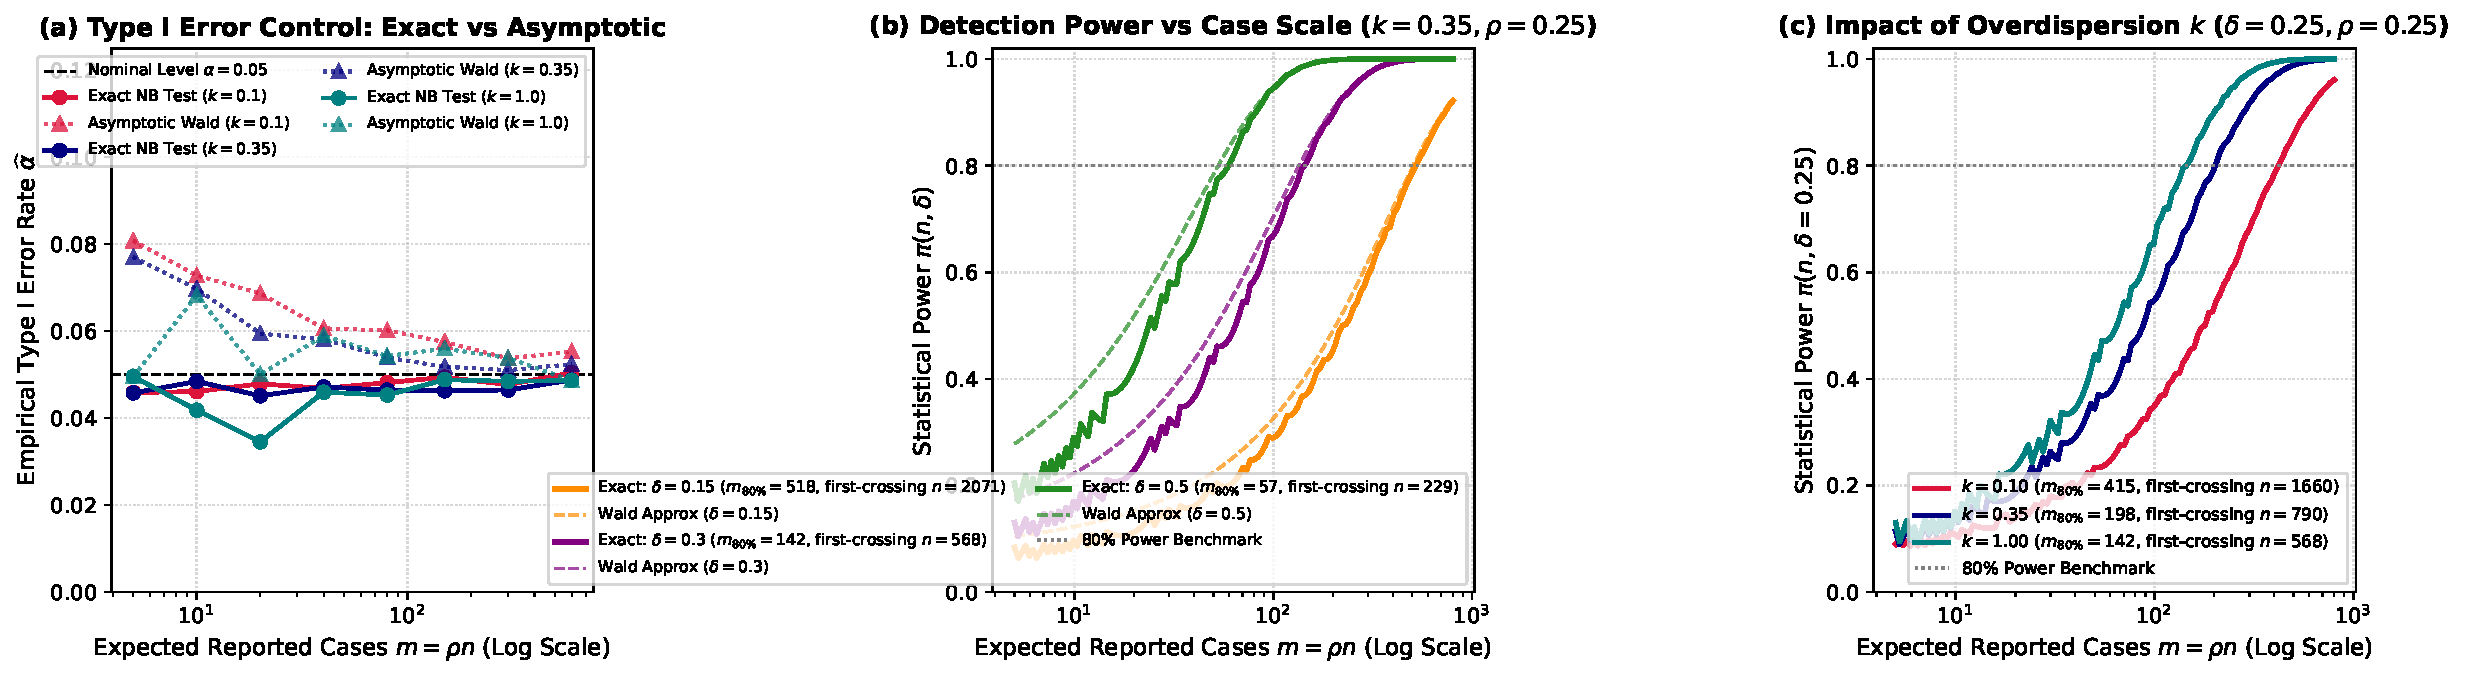
\includegraphics[width=\textwidth]{../figures/fig2_growth_detection_power.pdf}
\caption{\textbf{当期超临界增长判定检验功效与有限样本性质验证}（名义水平 $\alpha = 0.05$，基准 $\rho = 0.25$）。(a) 第一类错误率（Size）控制：渐近正态 Wald 检验（虚线）在低病例规模（$m < 40$）且严重超传播（$k=0.1$）时经验一类错误率最高达 8.1\%（$m=5$，30,000 次模拟），系统性高于名义水平，而精确负二项非随机化检验（实线）在全样本网格上严格控制错误率低于 0.05；(b) 检出功效曲线随备择强度 $\delta = R_t - 1$ 的提升，当 $k=0.35$ 时，达到 80\% 功效所需的期望报告规模由 $\delta=0.15$ 的 $m=517.8$（$n=2071$）下降至 $\delta=0.30$ 的 $m=142.0$（$n=568$）与 $\delta=0.50$ 的 $m=57.2$（$n=229$）；(c) 个体超传播离散度 $k$ 的冲击：在 $\delta=0.25$ 增长强度下，达到 80\% 检出功效所需的期望病例数从低异质性 $k=1.0$ 的 $m=142.0$（$n=568$）暴增至严重超传播 $k=0.1$ 的 $m=415.0$（$n=1660$），需求放大了近 3 倍。}
\label{fig:detection_power}
\end{figure}

模拟结果展现了三项重要发现：
\begin{enumerate}
\item \textbf{第一类错误率失真：} 如图~\ref{fig:detection_power}(a) 所示，渐近 Wald 检验在低病例规模下失效。在网格内最小规模 $m = 5$、$k = 0.1$ 处，Wald 检验的经验一类错误率达到最高的 8.1\%（30,000 次模拟），约为名义水平 0.05 的 1.6 倍，且全低规模段（$m < 40$）系统性过检，极易引发虚假超临界报警；相比之下，命题~\ref{prop:growth_test} 导出的离散精确临界值 $c_\alpha$ 在所有规模下均保守且严格受控于 0.05 以下。
\item \textbf{检出功效对备择强度的非线性响应：} 如图~\ref{fig:detection_power}(b) 所示，在固定 $k=0.35$ 时，达到 80\% 可靠功效所需的期望报告病例数随信号强度急剧下降：微弱增长（$\delta = 0.15$）需要 $m = 517.8$ 例；中度增长（$\delta = 0.30$）降至 $m = 142.0$ 例；显著增长（$\delta = 0.50$）仅需 $m = 57.2$ 例即可可靠检出。
\item \textbf{超传播对样本需求的放大机制：} 如图~\ref{fig:detection_power}(c) 所示，在相同增长信号（$\delta = 0.25$）下，个体异质性越强（$k$ 越小），曲线右移越显著。从低异质性 $k=1.0$ 到强超传播 $k=0.1$，$m$ 需求放大了近 3 倍。
\end{enumerate}

\subsection{时间序列更新过程：事后增长统计量与事前单步病例预测}\label{subsec:sim_forecasting}

在时间序列动态更新过程中，记预测时已知的历史报告加权和为：
\begin{equation}
D_t \triangleq \sum_{s=1}^S w_s C_{t+1-s}.
\end{equation}
当历史连续多周报告全部为零时，分母 $D_t = 0$ 导致比值无定义。在统计评估中，我们明确规定评估仅在具备活跃历史信息的周（$D_t > 0$）上进行。实测表明，在每组 150 条轨迹、每条 26 个预测起点（共 3,900 个评价点）中：在 $m=6$ 组中仅剔除 3 周（发生率 0.077\%，有效周数 3,897）；在 $m=12$ 组仅剔除 1 周（发生率 0.026\%，有效周数 3,899）；在 $m \ge 25$ 的所有规模组中剔除数为 0（有效周数均为 3,900）。需要特别指明：图~\ref{fig:forecasting_crossover} 横轴的 $m$ 表示每条轨迹的初始期望报告规模；由于在 $\bar{R}=1.15$ 下后续规模随传播过程动态变化，理论曲线仅作按初始规模排列的对比参照。

在此活跃周子集上，我们严格区分两个评价对象：
\begin{enumerate}[label=(\arabic*)]
\item \textbf{事后代理增长统计量误差：} 在 $t+1$ 期报告 $C_{t+1}$ 实际观测后，事后计算比值 $G_{t+1} \triangleq C_{t+1}/D_t$。其相对基础水平的均方误差定义为 $\mathbb{E}[(G_{t+1} - \bar{R})^2 \mid D_t > 0]$。
\item \textbf{事前单步病例预测相对均方误差（Ex-ante Forecasting RelMSE）：} 在 $t$ 时刻，决策者仅依据截至 $t$ 期的报告历史，对下一期报告病例数作出预测：$\widehat{C}_{t+1 \mid t} \triangleq \bar{R} D_t$。当 $C_{t+1}$ 实际出现后，计算相对均方预测误差：
\begin{equation}
\operatorname{RelMSE}(m) \triangleq \mathbb{E}\left[\left(\frac{C_{t+1} - \widehat{C}_{t+1 \mid t}}{\widehat{C}_{t+1 \mid t}}\right)^2 \;\middle|\; D_t > 0\right] = \frac{1}{\bar{R}^2}\mathbb{E}\left[(G_{t+1} - \bar{R})^2 \;\middle|\; D_t > 0\right]. \label{eq:relmse_identity}
\end{equation}
\end{enumerate}
式~\eqref{eq:relmse_identity} 表明：\textbf{在相同的活跃周样本上，事前病例预测相对误差与事后增长统计量误差严格相差常数因子 $1/\bar{R}^2$}。因此，二者在每一规模组的相对翻倍削减率中常数因子完全相消，经验降幅严格同一。

然而，\textbf{这一代数等价性并不证明它们在理论上精确等于单代理想基准}。设 $\mu_{t+1 \mid t} \triangleq \mathbb{E}[C_{t+1} \mid \mathcal{F}_t^C]$ 与 $\sigma_{t+1 \mid t}^2 \triangleq \operatorname{Var}(C_{t+1} \mid \mathcal{F}_t^C)$，在活跃周上有严格条件分解：
\begin{equation}
\mathbb{E}\left[(G_{t+1} - \bar{R})^2 \;\middle|\; D_t > 0\right] = \mathbb{E}\left[\frac{\sigma_{t+1 \mid t}^2}{D_t^2} + \left(\frac{\mu_{t+1 \mid t}}{D_t} - \bar{R}\right)^2 \;\middle|\; D_t > 0\right]. \label{eq:exact_renewal_decomp}
\end{equation}
式~\eqref{eq:exact_renewal_decomp} 清楚揭示了更新过程较之单代基准所增加的两个关键机制：其一是用报告历史代理真实感染压力导致的\textbf{预测偏差项} $(\mu_{t+1 \mid t}/D_t - \bar{R})^2$；其二是随机分母 $D_t$ 对条件方差的\textbf{倒数二次方重新加权}。

因此，由已知真实风险集单代模型导出的 $V(m) = v_R + A/m$ 以及经缩放的参照曲线 $(v_R + A/m)/\bar{R}^2$，\textbf{仅作为参照基准而非更新过程预测误差的精确定理}。二者的渐近环境底板分别为 $v_R = 0.040$ 与 $v_R / \bar{R}^2 = 0.0302$。

\begin{figure}[htbp]
\centering
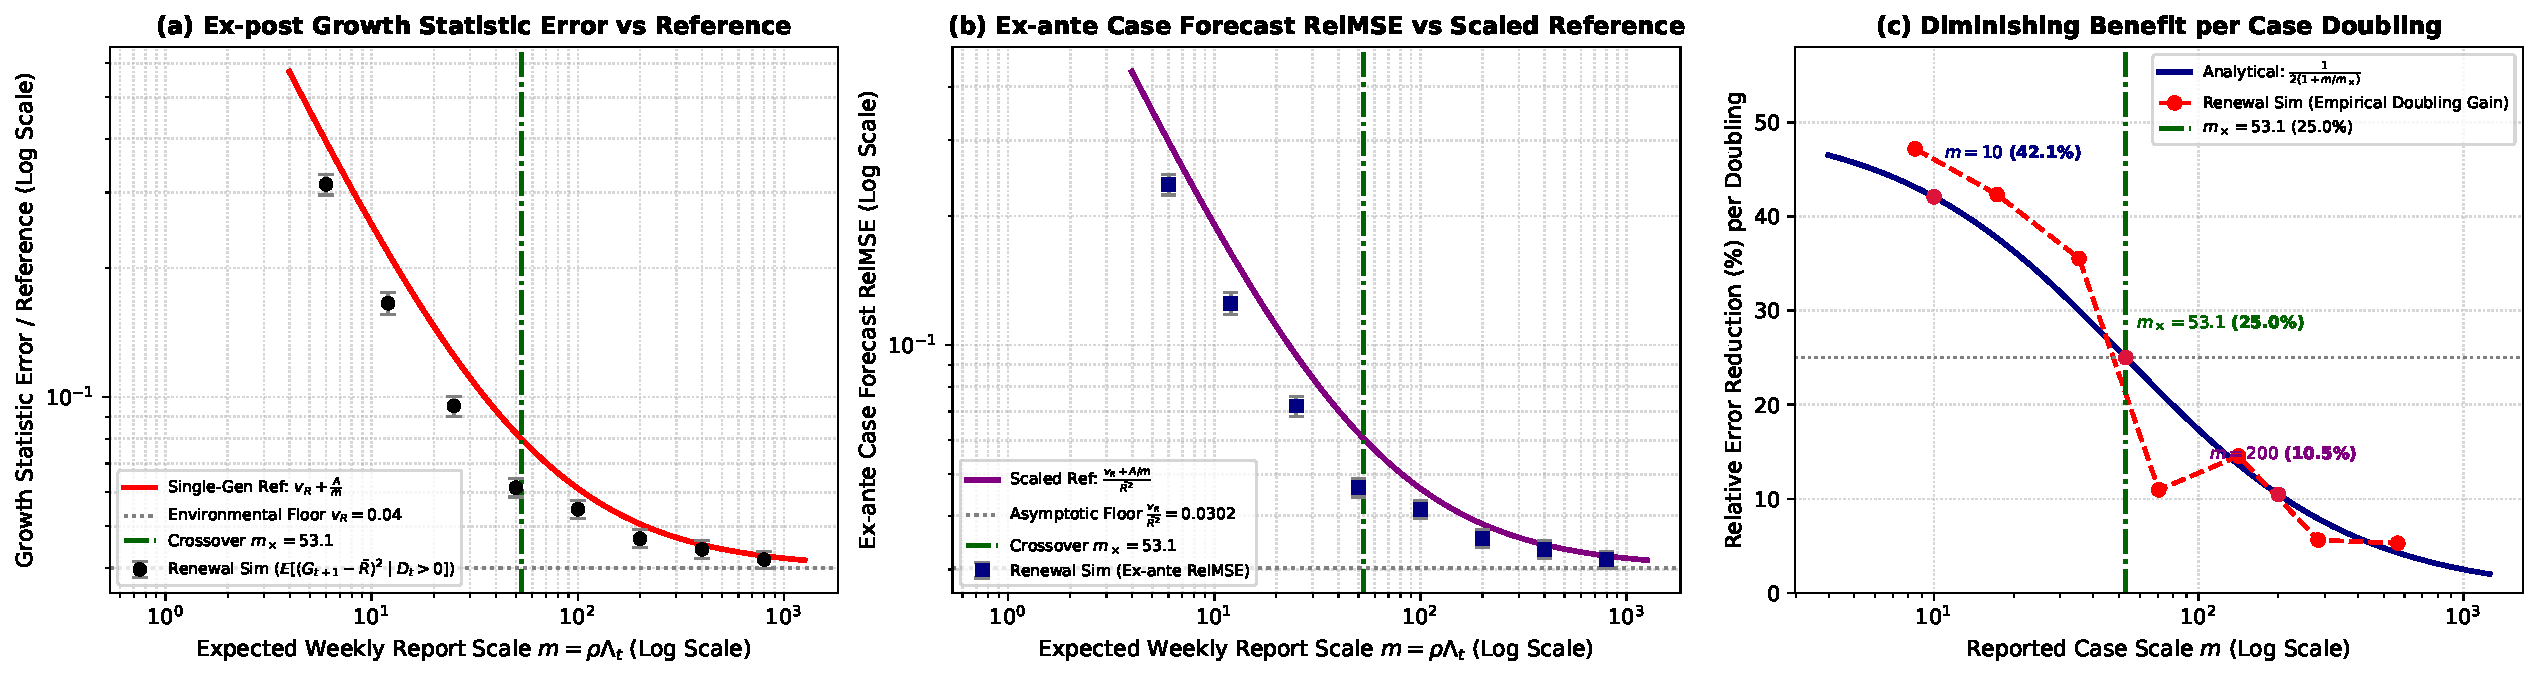
\includegraphics[width=\textwidth]{../figures/fig3_forecasting_saturation_crossover.pdf}
\caption{\textbf{更新过程时间序列事后增长统计量与事前单步病例预测误差对照}。(a) 事后代理增长统计量均方误差（黑色散点带 95\% 置信区间）与单代已知基准参照曲线 $V(m) = v_R + A/m$（红实线，其中 $A=2.1232, v_R=0.04$）的对照；(b) 事前单步病例预测相对均方误差（蓝色方块带 95\% 置信区间）与缩放参照曲线 $\frac{v_R + A/m}{\bar{R}^2}$（紫实线）紧密贴合；(c) 病例规模每翻一倍所带来的相对误差削减百分比：红圈为更新过程经验翻倍降幅（事后统计量与事前预测经验降幅严格同一），深蓝实线为理论解析公式 $\frac{1}{2(1 + m/m_\times)}$。在 $m=10$ 时，参照翻倍削减为 42.1\%；在交叉点 $m_\times = 53.1$ 处为 25.0\%；越过交叉点后，在 $m=200$ 时边际削减迅速衰减至 10.5\%。（样本说明：每规模组共 150 条轨迹 $\times$ 26 个预测起点 = 3,900 点；$m=6$ 组剔除 $D_t=0$ 者 3 点，有效 3,897 点；$m=12$ 组剔除 1 点，有效 3,899 点；$m \ge 25$ 各组有效点均为 3,900 点）。}
\label{fig:forecasting_crossover}
\end{figure}

数值实验结果展现了三项关键发现：
\begin{enumerate}
\item \textbf{事后统计量与参照曲线的高度协同：} 如图~\ref{fig:forecasting_crossover}(a) 所示，事后代理增长统计量虽然叠合了式~\eqref{eq:exact_renewal_decomp} 中的预测偏差与随机分母波动，但其随规模衰减形态紧密依循单代参照曲线 $v_R + A/m$。在极小规模（$m=6$）下，经验均方误差（0.313）与单代参照值（0.394）存在一定数值差异，其来源涉及动态风险集的时序漂移、随机分母加权及活跃周的截断筛选；但随着规模增加，经验误差平滑趋向环境方差底板 $v_R = 0.040$。
\item \textbf{事前预测相对误差的严格对应：} 如图~\ref{fig:forecasting_crossover}(b) 所示，在 $t$ 时刻给出的病例预测相对均方误差，其经验曲线在全尺度范围内平滑追踪缩放参照曲线 $\frac{v_R + A/m}{\bar{R}^2}$，渐近收敛于环境相对方差 $v_R / \bar{R}^2 = 0.0302$。
\item \textbf{边际削减收益的定量衰减规律：} 针对解析参照曲线 $V(m) = v_R + A/m$，病例规模翻倍时的相对方差下降比例严格由下式给出：
\begin{equation}
\frac{V(m) - V(2m)}{V(m)} = \frac{1}{2(1 + m/m_\times)}.
\end{equation}
如图~\ref{fig:forecasting_crossover}(c) 所示，在 $m_\times \approx 53.1$ 下，当 $m = 10$ 时，规模翻倍可降低约 42.1\% 的解析方差；越过交叉点 $m_\times = 53.1$（此处理论边际收益为 25.0\%）后，当 $m = 200$ 时，病例规模再翻倍仅能带来约 10.5\% 的方差削减。这印证了本文的核心直觉：\textbf{越过交叉点后，扩大病例捕获依然能边际改善预测，但由于环境扰动占主导，其改善速率急剧放缓}。
\end{enumerate}

\subsection{数值实验复现规格与参数说明}\label{subsec:sim_reproducibility}

为确保所有模拟数值与图表的高度可复现性，本节列明复现规格：
\begin{enumerate}[label=(\alph*)]
\item \textbf{软件包与离散分布参数化：} 全部算法基于 Python 3.10 与 \texttt{scipy.stats} 实现。负二项分布采用标准形式 $\operatorname{NB}(r, p)$，其中在条件均值 $\mu = \rho n R$ 与离散参数 $k$ 下，参数映射为 $r = nk, p = \frac{k}{k + \rho R}$。累积尾概率由生存函数 \texttt{stats.nbinom.sf(c - 1, r, p)} 计算。
\item \textbf{图 2 离散功效与样本量枚举规则：} 随机数种子设定为 20260924。对给定 $(k, \rho, \alpha=0.05)$，临界值 $c_\alpha$ 通过整数搜索使零假设生存概率首次不超过 $\alpha$。在备择假设 $R_t = 1 + \delta$ 下，自 $n=1$ 起以步长 1 递增枚举整数 $n$，取首次满足功效 $\pi(n, \delta) \ge 0.80$ 的最小整数 $n$，并换算为期望报告规模 $m = \rho n$。
\item \textbf{图 3 更新过程仿真参数与分母：} 随机数种子设定为 20260925。感染间隔采用 4 周离散核 $w = (0.45, 0.35, 0.15, 0.05)$，环境扰动采用 Gamma 分布采样，均值为 $\bar{R}=1.15$，方差为 $v_R=0.04$。每规模组评估 150 条轨迹，时间跨度 $T=30$（前 4 周作为启动核，预测评估周为 $t=4$ 至 29 共 26 周），总评价周数分母为 3,900。
\end{enumerate}

\section{实证检验：全美流感住院监测数据（2020--2026）}\label{sec:empirical}

为对本文提出的理论方差结构、饱和交叉点 $m_\times$、报告杠杆冲击以及反证边界提供真实流行病学监测环境下的检验，本节利用全美疾控中心国家医疗保健安全网（CDC NHSN）周度流感住院报告数据开展系统实证。

\subsection{数据源、制度分段与数据预处理}\label{subsec:emp_data}

数据来自全美各州及华盛顿特区医院向 CDC NHSN 上报的周度实验室确诊新发流感住院人数（\texttt{Total Influenza Admissions}）及各州周度医院报告覆盖率（字段名 \texttt{Percent Hospitals Reporting Influenza Admissions}）。样本时间跨越 2020 年 8 月至 2026 年 9 月，涵盖 50 个州及华盛顿特区共 16,218 个州--周观测。样本筛选采用单一口径：\textbf{$D_t \ge 5$ 的活跃周阈值}，得 10,303 个州--周有效样本；本文第~\ref{subsec:emp_early}--\ref{subsec:emp_spatial} 节的全部主分析、稳健性与滚动核验均基于该口径，不另设覆盖率门槛（避免系统性剔除低覆盖观测）。在此口径下三个报告制度阶段的医院平均填报覆盖率分别为 91.1\%、54.6\% 与 91.8\%，自愿过渡期的覆盖率断崖式跌落构成本文考察报告率冲击的主要制度变异来源。

\paragraph{报告制度三阶段划分：}
该监测系统在样本期内经历了三次具有政策调整特征的制度切换：
\begin{enumerate}[label=(\arabic*)]
\item \textbf{前过渡高覆盖期（数据起点 2020 年 10 月至 2024 年 4 月 30 日，共 184 个有效周、$N = 6{,}009$）：} 该时段合并了两个制度子段——2020 年 10 月至 2022 年 9 月的大流行早期高强度上报（$N = 2{,}627$，平均覆盖率 87.8\%）与 2022 年 10 月 NHSN 法定强制上报起的法定强制段（$N = 3{,}382$，平均覆盖率 93.7\%），两子段合计平均覆盖率 91.1\%（中位数 92.3\%）；第~\ref{subsec:emp_policy} 节的离散度对照将以法定强制段单列报告；
\item \textbf{第二阶段（自愿过渡期，2024 年 5 月 1 日至 2024 年 10 月 31 日，26 个有效周、$N = 420$）：} 强制令随紧急状态解除到期，医院转为自愿填报，各州平均报告覆盖率断崖式跌落至 54.6\%（中位数 45.7\%）；
\item \textbf{第三阶段（CMS 新规重制期，2024 年 11 月 1 日起至样本终点 2026 年 8 月，96 个有效周、$N = 3{,}874$）：} 美国医疗保险与医疗补助服务中心（CMS）将呼吸道传染病数据上报重新作为医保定点医院资质条件，各州报告覆盖率迅速恢复至 91.8\%（中位数 93.2\%）。
\end{enumerate}

\paragraph{状态空间设定与观测对象界定：}
在离散周度时间序列中，取滞后权重向量 $w = (0.65, 0.25, 0.10)$（滞后 1、2、3 周，平均回溯延迟为 $\sum_{s=1}^3 s w_s = 1.45$ 周，约 10.2 天）构建各州第 $t$ 周的历史有效输入压力：
\begin{equation}
D_{j,t} = \sum_{s=1}^3 w_s C_{j, t+1-s}.
\end{equation}
这里的 $w$ 是\textbf{感染代际分布与住院报告延迟分布的离散复合卷积核}：从暴露感染、发病就医到收治入院并录入系统，普遍存在 5--10 天的临床与填报时滞，该卷积核把生物学代际结构（约 2.5--3.5 天）映射到周度住院观测的时间尺度上，使 $G_{j, t+1} = C_{j, t+1}/D_{j,t}$ 成为住院维度增长动力学的正确代理（Proxy of Hospitalization Growth）。当 $D_{j,t} \ge 5$ 时进入有效推断样本集（单一活跃周口径，不设覆盖率门槛，理由见第~\ref{subsec:emp_data} 节）。

\paragraph{阶段条件化预测基准与识别限定：}
本节在评估预测误差时，采用阶段条件化基准设定 $\widehat{C}_{j, t+1 \mid t} \triangleq \bar{R}_{\text{phase}} D_{j,t}$，评分口径取相对尺度均方误差——相对误差评分在传染病预测评估中具有避免大流行周主导加权的光照尺度优势 \citep{bosse2023scoring}——在控制跨期趋势参数变化的同等基准下，估计病例捕获规模 $D_t$ 与相对预测误差的条件关联。医院维度的填报覆盖率（比例）在微观机制上对应理论中的报告率杠杆 $\rho$，2024 年的制度切换由此构成命题~\ref{prop:levers_asymmetry} 的天然对照场景，其解释边界在第~\ref{subsec:emp_policy} 节结合季节性子样本进一步校准。

\begin{figure}[htbp]
\centering
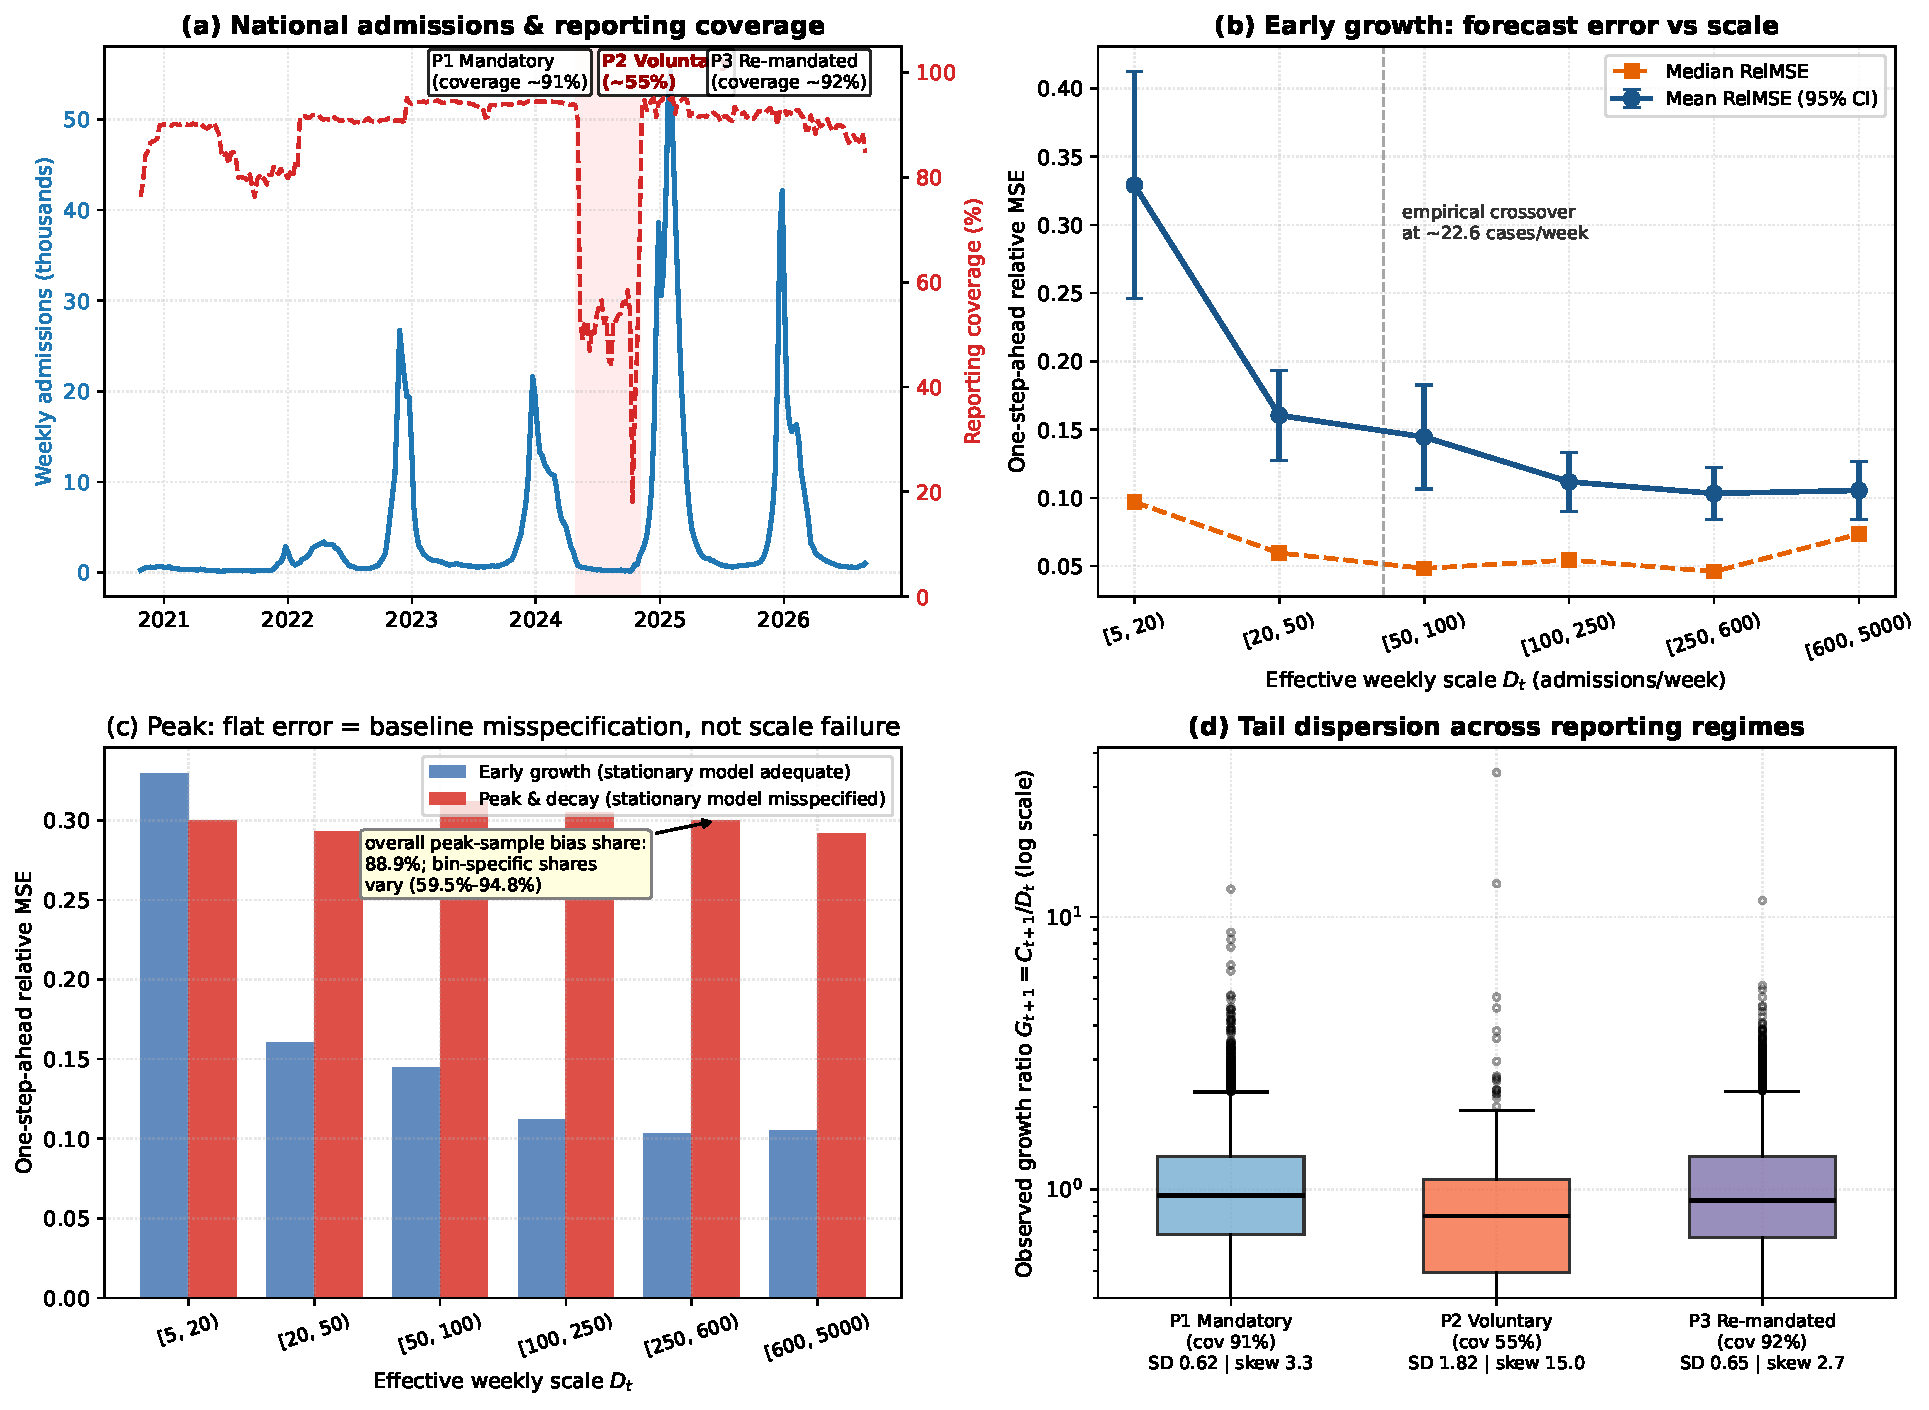
\includegraphics[width=\textwidth]{../figures/fig4_empirical_falsification.pdf}
\caption{\textbf{全美 CDC NHSN 流感住院真实监测数据实证与反证边界检验}。(a) 全美周度流感住院总人数（蓝实线，左轴）与各州医院平均填报覆盖率（红虚线，右轴）演变，阴影区域标示 2024 年 5--11 月报告覆盖率骤降的自愿过渡期；(b) 流行初期上升波段中，单步预测相对均方误差随每周病例捕获规模 $D_t$ 的衰减关系（蓝圆点为经验均值与 95\% CI，橙方块为中位数），误差在 $D_t \in [50, 250]$ 区间快速下降后进入约 0.103 的经验平台——对应经验损失曲线截距 $a$（与规模无关误差项）的主导区；(c) 达峰与回落期：以流行初期估计的平稳基准 $\bar{R}_{\mathrm{early}}=1.6706$ 预测全部阶段时，达峰与回落期（红柱）的总误差在所有规模组恒定处于 0.292--0.312 区间，看似不再随 $D_t$ 增大而下降；但达峰期总体样本的均值偏移项占总损失 88.9\%（0.267；各规模箱占比 59.5\%--94.8\% 不等），控制基准偏移后规模相关方差项仍显著为正，故失效的是跨期平稳基准假定而非病例规模本身；(d) 报告制度切换对观测离散度的冲击箱线图：自愿填报期标准差由 0.624 升至 1.823（扩张 192.1\%），偏度由 3.29 升至 14.98，恢复强制后两者回落至 0.649 与 2.68。}
\label{fig:empirical_validation}
\end{figure}

\subsection{检验一：流行初期波段的方差衰减与经验收益放缓平台}\label{subsec:emp_early}

按照第~\ref{sec:methods} 节关于基准模型适用边界的定义，我们在三个流感季节中提取\textbf{流行初期上升波段（Early Growth Phase）}：2022--2023 季的 10 月 8 日至 11 月 26 日；2023--2024 季的 10 月 14 日至 12 月 16 日；2024--2025 季的 11 月 9 日至 1 月 18 日。在这些波段内，人群对当年毒株的自发防护行为尚未全面激活，公共卫生干预尚未强力介入，传播环境相对平稳。此阶段有效样本（$N = 1267$）平均增长率为 $\bar{R}_{\mathrm{early}} = 1.6706$（标准差 0.7116）。\textbf{口径声明：}本节主分析以该阶段的 $\bar{R}_{\mathrm{early}}$ 为基准，属于\textbf{回顾性的阶段条件误差分析}——其目的是在受控的同等基准下检验误差随规模的衰减形态，而非声称该基准在波段内每个时点均可实时获得。严格的滚动起点预测（每个 $t$ 仅用其前数据估计基准）在第~\ref{subsec:emp_early} 节末单独报告，作为对规模效应结论的事前口径核验。

表~\ref{tab:empirical_scale} 报告了各规模分组下\textbf{回顾性阶段条件基准下的单步相对平方误差}的经验统计量。为考虑同州跨周的时间相关性与组内聚类不确定性，表中同时给出常规 SEM 与按州（State）聚类的稳健标准误（Cluster-robust SE）；本文的区间推断一律以州聚类 95\% 置信区间为准。

\begin{table}[htbp]
\centering
\caption{\textbf{全美流感住院流行初期波段单步预测误差随周捕获规模的分组统计}}
\label{tab:empirical_scale}
\small
\setlength{\tabcolsep}{3.8pt}
\begin{tabular}{lrrrrrr}
\toprule
每周有效规模 $D_t$ & 样本数 $N$ & 相对均方误差 & 中位数 & 普通 SEM & 州聚类 SE & 州聚类 95\% 置信区间 \\
\midrule
$[5, 20)$   & 319 & 0.3292 & 0.0969 & 0.0425 & 0.0437 & $[0.2435, 0.4149]$ \\
$[20, 50)$   & 297 & 0.1605 & 0.0596 & 0.0169 & 0.0189 & $[0.1235, 0.1974]$ \\
$[50, 100)$   & 187 & 0.1446 & 0.0483 & 0.0194 & 0.0198 & $[0.1057, 0.1835]$ \\
$[100, 250)$   & 220 & 0.1118 & 0.0545 & 0.0110 & 0.0114 & $[0.0895, 0.1341]$ \\
$[250, 600)$   & 152 & 0.1032 & 0.0460 & 0.0097 & 0.0133 & $[0.0771, 0.1293]$ \\
$[600, 5000)$   & 92 & 0.1054 & 0.0735 & 0.0109 & 0.0146 & $[0.0769, 0.1340]$ \\
\bottomrule
\end{tabular}
\end{table}

实证数据呈现出与理论命题~\ref{prop:trend_var} 高度吻合的边际衰减特征。
为使检验贴合理论的函数形式，我们不做分箱均值的目视比较，而是按式~\eqref{eq:var_prop2} 重写为 $v_R + A/m$ 后的形状，直接对原始观测估计仿射模型：
\begin{equation}
\mathbb{E}\!\left[\left(\frac{G_{t+1} - \bar{R}_{\mathrm{early}}}{\bar{R}_{\mathrm{early}}}\right)^{2}\ \middle|\ D_t\right] = a + \frac{b}{D_t}, \label{eq:affine_empirical}
\end{equation}
其中 $a$ 为\textbf{经验损失曲线的截距}——在该预测基准与规格下与规模无关的误差项，其与环境方差 $v_R$ 的机制对应有待微观参数识别；$b$ 为\textbf{经验规模相关项}，仅当接受 $a \leftrightarrow v_R$、$b \leftrightarrow A$ 的机制类比时，$b/a$ 才可读作理论交叉点的经验对应物，本文以下统一称其为\textbf{经验交叉点}。估计采用一阶可行广义最小二乘（FGLS）：由 OLS 起步，以拟合值平方的倒数为权重迭代至收敛，以应对相对均方误差的强异方差。标准误与置信区间由按州聚类的 cluster bootstrap 给出（1,500 次重抽）。
\begin{enumerate}
\item \textbf{规模相关方差项显著为正：} 仿射模型估计给出 $b = 2.2434$，按州聚类的 bootstrap 95\% 置信区间为 $[1.5019, 3.0161]$，1,500 次重抽样中无一次出现 $b \le 0$。这与式~\eqref{eq:var_prop2} 中病例规模相关方差项 $A/m$ 的递减形态相容，且不依赖分箱均值的目视趋势。从极小规模 $[5, 20)$（平均 RelMSE = 0.3292）扩大至 $[20, 50)$（0.1605），经验相对均方误差下降了 \textbf{51.3\%}；即使采用州聚类 95\% 置信区间，$[5, 20)$ 的下界（0.2435）与 $[20, 50)$ 的上界（0.1974）仍严格分离；
\item \textbf{经验方差底板与经验交叉点：} 仿射拟合的截距给出 $a = 0.0991$（95\% CI $[0.0841, 0.1173]$），即病例规模趋于无穷时经验相对均方误差的下限；按上述类比其对应理论的环境方差底板 $v_R$，但这是机制解读而非参数识别。由 $m_\times^{\mathrm{emp}} = b/a$ 得经验交叉点 $22.6$（95\% CI $[13.7, 33.7]$）例/周。该估计对规格选择的敏感性呈分化：十分位组均值拟合（以降低 $D_t$ 自身测量误差的影响）给出与基准一致的 $22.6$；但剔除损失最大的 1\% 观测后交叉点明显左移至 $10.6$，表明其对尾部处理有实质敏感性，应视为量级估计而非点位识别。针对 $D_t$ 与 $C_{t+1}$ 共享报告噪声导致的变量误差问题，我们进一步以滞后 3--5 周报告序列另行构造的工具规模 $D_t^{\mathrm{iv}}$ 做两阶段最小二乘对照（有效样本 $N = 1{,}051$；工具的关键假定是滞后核仅通过规模 $D_t$ 影响当期损失；持续传播态势、季节性与填报行为若同时关联滞后核与当期损失，会削弱该对照的排除力，故其结果应读作方向性敏感性检验而非严格识别）：$b$ 的估计为 $2.5305$（$a = 0.0841$），与 FGLS 基准（$2.2434$）点估计方向一致；因排除限制未获验证，该对照不能据此识别或界定测量误差偏倚——只能说点估计仍为正、与基准方向一致。需强调：$m_\times^{\mathrm{emp}}$ 定义在\textbf{住院维度的周捕获规模} $D_t$ 上，而理论交叉点 $m_\times = \frac{\bar{R} + \rho(\bar{R}^2 + v_R)/k}{v_R}$ 定义在微观期望报告病例数 $m = \rho n$ 上，两者并非同一量。在呼吸道病毒住院的典型参数空间下（$k \approx 0.2 \sim 0.5$、住院捕获率 $\rho \approx 0.01 \sim 0.05$、周度环境方差 $v_R \approx 0.04 \sim 0.08$），理论公式导出数十至百例量级，与经验值的十至数十例\textbf{同阶但不等同}；这种同阶相容性为理论尺度提供了外部效度支持，也为后续微观计量标定划定了明确的参数空间。

\end{enumerate}

\paragraph{过度离散随规模的衰减：} 分箱计算 loss 的方差--均值比可见，$\operatorname{Var}(L)/\mathbb{E}[L]^2$ 从 $[5,20)$ 箱的 5.32 单调下降至 $[600,5000)$ 箱的 0.99。这与式~\eqref{eq:var_prop2} 的预测一致：当规模相关方差项 $A/m$ 衰减后，剩余的方差主要由不随规模变化的环境项主导，超额离散随之收缩。这一形态也为 FGLS 采用 $1/\hat{\mu}^2$ 权重提供了依据。

\paragraph{事后选定初期波段内的滚动起点核验：} 上述主分析属回顾性口径。为核验规模效应结论在事前信息集下是否保持，我们对初期波段（波段本身为事后指定）每个观测 $t$ 改用\textbf{仅其前数据}估计的基准重算损失：全部历史扩张窗（$N=1267$）得 $b = 9.1579$（聚类 bootstrap 95\% CI $[5.8168, 12.8750]$），$b/a = 22.5$；26 周滚动池（$N=1267$）得 $b = 9.4562$（CI $[6.7612, 12.8078]$），$b/a = 42.7$；逐州扩张窗（$N=1260$）得 $b = 13.2666$（CI $[9.1385, 18.2948]$），$b/a = 38.9$；三者的 $a$ 分别为 0.4063、0.2217、0.3409。三种滚动规格下误差水平整体抬升（$a$ 从 0.099 升至 0.22--0.41）——回顾性基准确实偏乐观，其份额分解应理解为\textbf{同等基准下的机制拆解而非可实现的预测精度}；但规模相关项在所有事前口径下均显著为正、分箱误差保持单调下降，大规模端（$D_t \ge 250$）实际观测的误差水平也稳定低于全体平均的四至六成。规模效应的存在性与方向经受住了事前信息集的检验；变化的只是误差的绝对水平与份额结构。

\paragraph{误差预算分解：} 仿射拟合不仅给出参数，还允许把初期波段的平均相对均方误差（0.181）直接分解为拟合值的代数分解份额：与规模无关的拟合项 $a$ 贡献 \textbf{54.6\%}，规模相关项 $b/D_t$ 贡献 \textbf{45.1\%}，模型外残差不足 0.3\%。作为对照，样本中实际处于大规模端（$D_t \ge 250$，越过经验交叉点 22.6 一个量级，共 244 个观测）的组内平均相对均方误差为 0.104——与拟合截距 $a = 0.0991$ 数值一致（该一致性仅表明截距对应样本内大规模观测的已实现水平，不构成对其机制来源的识别），即经验数据中已实现的大规模观测误差水平约为全体平均（0.181）的六成；其余约五成半的误差份额落在与规模无关的拟合项上，提示环境协变量采集与多期平滑是值得进一步评估的互补路径（命题~\ref{prop:budget_tradeoff}）。达峰期条件方差口径下的分解结构类似（46.7\% 对 55.6\%）。这组份额结构给本文的核心问题提供了一个可操作的参照：规模收益真实存在，但过半误差份额与规模无关，监测资源的配置取决于当前所处份额结构，而非无条件的"越多越好"。

\subsection{检验二：达峰与回落期——失效的是平稳基准而非病例规模}\label{subsec:emp_falsification}

科学命题的成立必须伴随明确的证伪边界，但证伪检验本身必须可解释。本文的反证检验采取如下口径：\textbf{用流行初期估计的平稳基准 $\bar{R}_{\mathrm{early}}$ 去预测全部阶段的病例}。此时总误差可分解为两部分：其一是\textbf{基准偏移造成的常数偏差} $\left(\bar{R}_{\mathrm{early}}-\bar{R}_{\mathrm{phase}}\right)^2/\bar{R}_{\mathrm{early}}^2$，它与病例规模无关；其二是该阶段内部的\textbf{条件方差}，只有后者才回答“规模是否还有用”。若只报告总误差，则“误差不随规模下降”可能是常数偏差主导的平凡结果，不构成对规模有效性的检验。因此下文两者分别报告。达峰与回落阶段定义为各流感季全国达峰周（2022-12-03、2023-12-30、2025-02-08）及其随后 7 周，共 1220 个州--周。在此期间，全美各州平均增长率骤降至 $\bar{R}_{\mathrm{peak}} = 0.8075$（标准差 0.3048），远低于流行初期的 1.6706。

表~\ref{tab:peak_stationary} 与图~\ref{fig:empirical_validation}(c) 给出了该口径下的分组误差。

\begin{table}[htbp]
\centering
\caption{\textbf{达峰与回落期：以平稳基准 $\bar{R}_{\mathrm{early}}$ 预测时的分组误差}}
\label{tab:peak_stationary}
\small
\setlength{\tabcolsep}{3.8pt}
\begin{tabular}{lrrr}
\toprule
每周有效规模 $D_t$ & 样本数 $N$ & 相对均方误差 & 中位数 \\
\midrule
$[5, 20)$ & 33 & 0.2998 & 0.2361 \\
$[20, 50)$ & 140 & 0.2927 & 0.2591 \\
$[50, 100)$ & 162 & 0.3120 & 0.3085 \\
$[100, 250)$ & 312 & 0.3049 & 0.3005 \\
$[250, 600)$ & 311 & 0.2998 & 0.2976 \\
$[600, 5000)$ & 262 & 0.2916 & 0.2987 \\
\bottomrule
\end{tabular}
\end{table}

对比两个阶段可以发现强烈的非对称性：
\begin{itemize}
\item \textbf{总误差层面：} 以平稳基准预测时，达峰与回落期的误差在所有规模组恒定处于 0.292--0.312，从 $[5, 20)$ 组的 0.2998 到 $[600, 5000)$ 组的 0.2916 几乎没有下降；
\item \textbf{但这一平稳性主要是常数偏差所致：} 在达峰期\textbf{总体样本}的均值--方差分解中，基准偏移项 $\left(\bar{R}_{\mathrm{peak}} - \bar{R}_{\mathrm{early}}\right)^2/\bar{R}_{\mathrm{early}}^2 = 0.2669$，占总体损失的 88.9\%。须注意这是总体口径的份额：按各箱自身均值计算的偏差占比随规模上升（$[5,20)$ 箱 59.5\% 至 $[600,5000)$ 箱 94.8\%），小规模箱的偏差占比明显更低、条件方差占比更高，故总体份额不代表各规模箱具有相同的偏差结构；
\item \textbf{条件方差层面：} 改用达峰期自身的均值 $\bar{R}_{\mathrm{peak}}$ 作基准后，仿射拟合给出 $a = 0.0665$（95\% CI $[0.0467, 0.0897]$）、$b = 7.9272$（95\% CI $[5.4239, 11.2248]$）——达峰期内部规模相关项显著为正。\textbf{但阶段间的 $b$ 比较必须统一损失尺度}：本条的达峰期损失以 $\bar{R}_{\mathrm{peak}} = 0.8075$ 归一化，而初期损失以 $\bar{R}_{\mathrm{early}} = 1.6706$ 归一化，两个 $b$ 不在同一分母上。表~\ref{tab:stage_scales} 报告三种口径下的阶段比较：在\textbf{共同分母（$\bar{R}_{\mathrm{early}}$）}与\textbf{未归一化}两种可比口径下，达峰期的 $b$（1.8521 与 5.1690）均\textbf{低于}初期（2.2434 与 6.2611）；为使推断完整，我们在同一样本、共同分母口径下估计了四种规格的两阶段斜率差：分别 OLS（$2.3049$ 对 $1.3866$，差 $-0.9183$）、联合 OLS 交互项（$-0.9183$；按州聚类 bootstrap 95\% CI $[-2.2702, 0.6261]$）、分别 FGLS（$2.2434$ 对 $1.8521$，差 $-0.3913$）、联合 FGLS 交互项（$-0.3913$）。两种估计程序内，联合交互项均精确等于分别拟合的斜率差（代数恒等），差异只发生在 OLS 与 FGLS 之间——源于 FGLS 迭代权重随拟合值重新估计。全部四种规格的置信判断一致：阶段斜率差点估计为负但区间含零，未发现达峰期斜率增强，也不能断言其更低。共同支撑集 $[50,600)$ 上结论相同（共同分母口径 1.6326 对 2.9264）。原稿若以各自归一化口径直接比较（7.9272 对 2.2434）会得出"达峰期规模项绝对量更高"的相反印象，那是分母差异的伪象；

\begin{table}[htbp]
\centering
\caption{\textbf{两阶段规模相关项 $b$ 的三口径比较}}
\label{tab:stage_scales}
\small
\setlength{\tabcolsep}{4pt}
\begin{tabular}{lrrl}
\toprule
损失口径 & 初期 $b$ & 达峰期 $b$ & 回答的问题 \\
\midrule
未归一化 $(G-\bar{R}_{\mathrm{phase}})^2$ & 6.2611 & 5.1690 & 增长代理的绝对误差规模 \\
共同分母 $\bar{R}_{\mathrm{early}}^2$ 归一化 & 2.2434 & 1.8521 & 同一相对尺度下的阶段差异 \\
各阶段均值归一化 & 2.2434 & 7.9272 & 各阶段相对自身基准的误差 \\
\bottomrule
\end{tabular}
\end{table}

\item \textbf{因此正确的反证结论是关于基准而非样本量：}在疫情高峰与回落期，人群行为改变、节假日填报积压及医疗系统挤兑使\textbf{跨期平稳基准} $\bar{R}$ 不再适用，单期预测的首要误差来源转为基准偏移，这解释了平稳模型在达峰期近 88.9\% 的总体误差贡献。但本文的检验\textbf{不支持}"达峰期病例规模不再有用"这一更强主张：控制基准偏移后，达峰期内部的规模相关项仍显著为正（$b = 7.9272$，95\% CI $[5.4239, 11.2248]$）。同时，统一尺度后的比较表明达峰期的规模项\textbf{并不比初期更强}（表~\ref{tab:stage_scales}）——规模在两阶段同样有用，但未显示阶段间增强。实际含义是：达峰期需要换用\textbf{非平稳状态模型或显式行为协变量}，而不是停止扩大病例捕获。
\end{itemize}

\paragraph{时变经验交叉点的探索性证据：} 上述两阶段对比（初期 $b/a = 22.6$ 对达峰期 $119.2$）提示经验交叉点可能随疫情阶段移动。为考察这一点，我们对全部有效观测做 26 周滚动窗口的窗口条件化仿射拟合（窗口内以自身均值 $\bar{R}_w$ 为基准）。251 个窗口的经验交叉点中位数为 36.5（IQR $[14.2, 61.6]$），量级与分段估计一致，但离季窗口的估计极不稳定（个别窗口逾千例）；须注意逐周滚动产生的高度重叠窗口使该 IQR 的有效样本量小于表观窗口数，区间解读应视为保守。为考察窗口内基准与窗口误差同源的影响，我们改用\textbf{前一窗口的均值作滞后基准}重估（滞后只保证时间先后，不自动保证外生性）：流感季窗口中位数 19.7 对非流感季 47.9，与窗口内基准下的分离（20.4 对 46.9）基本一致，说明该阶段性分离并非窗口内基准机械压缩的产物。稳健的定性事实是：\textbf{经验交叉点不是常数}——在传播活跃期规模收益的边界更近、扩大捕获更早进入回报放缓区，而低发期则需要更大的规模才能逼近环境底板，为动态监测资源配置提供了直接可用的阶段信号。

\subsection{检验三：报告制度切换对观测噪声的冲击（命题 3 的实证启示）}\label{subsec:emp_policy}

2024 年 5 月至 10 月的自愿填报过渡期为观察报告率波动下的噪声表现提供了现实场景。为避免系统性剔除低覆盖率观测，本节的有效样本仅要求 $D_t \ge 5$，不对医院覆盖率设门槛。如图~\ref{fig:empirical_validation}(d) 所示：
\begin{itemize}
\item 在前过渡高覆盖期全段（$N = 6{,}009$，平均覆盖率 91.1\%）观测周度增长率 $G_{t+1}$ 的标准差为 0.624、偏度 3.29；其	extbf{法定强制子段}（2022 年 10 月起，$N = 3{,}382$，覆盖率 93.7\%）单列为标准差 0.620、偏度 3.45——与全段几乎相同，说明早期高覆盖子段（标准差 0.628）不驱动该期离散度；
\item 在第二阶段自愿填报期（$N = 420$，平均覆盖率跌至 54.6\%），观测增长率的标准差攀升至 \textbf{1.823}（增加 \textbf{192.1\%}），偏度从 3.29 暴增至 \textbf{14.98}，最大值达到 33.9（为强制期的 2.7 倍）；四分位距则由 0.638 变为 0.594；
\item 在第三阶段 CMS 恢复强制后（$N = 3{,}874$，覆盖率回升至 91.8\%），观测增长率的标准差迅速回落至 0.649，偏度回落至 2.68——与	extbf{法定强制子段}的 0.620/3.45 相比几乎完全恢复，且此对照两端（0.620 与 0.649）同为法定强制制度，阶段可比性最严格。
\end{itemize}
\paragraph{离散度指标的选择与解释边界：} 自愿填报期观测增长率的离散度扩张\textbf{并非在所有稳健离散度指标上都成立}：标准差扩张 192.1\%、偏度扩张 355.3\%，但四分位距（0.638 $\to$ 0.594）与中位绝对离差（0.298 $\to$ 0.299）基本不变。这说明覆盖率下降主要放大的是\textbf{分布的右尾与极端值}，而非主体分布的宽度。此外，自愿过渡期（5--10 月）恰逢流感夏季低发期，样本中仅 55 个州--周落在流感季；在流感季子样本中，自愿期标准差为 4.793、IQR 为 1.818，均高于强制期（0.652 与 0.710），方向与全样本一致。两个证据方向的一致性——全样本与流感季子样本（自愿期标准差 4.793 对强制期 0.652）同向放大，且尾部指标与主体指标明确分化——与\textbf{报告率冲击放大分布右尾}的理论机制方向相容；鉴于医院维度覆盖率并不等同于事件级二项报告概率、停止填报的医院可能非随机（规模、季节、住院结构皆可混杂），且自愿期与夏季低发期重叠，本节对比定位为\textbf{与漏报噪声机制相容的描述性证据}，而非制度冲击的因果检验。

\subsection{检验四：空间跨区域汇聚的方差收益与异质性限制}\label{subsec:emp_spatial}

最后，针对通过地理汇聚扩大基数 $n$ 的效果，我们将 50 个州及华盛顿特区的数据按周加总，构建全美整体流感住院时间序列。在全美汇总序列的流行初期波段中，平均周捕获规模为 $D_t \approx 6662$ 例，单步预测相对均方误差骤降至 \textbf{0.0348}（中位数 0.0115，$N = 28$），显著低于任何单个大州所达到的经验平台（$\sim 0.10$）。全国汇总序列在该评分下误差较低这一事实，说明空间汇聚与更低的相对误差并存；将其归因于"各州未完全同步的局部环境扰动相互抵消"与命题~\ref{prop:levers_asymmetry} 中"唯有扩大真实基数才能使各项方差同时衰减"的方向相容，但本对比未单独识别环境抵消、子代波动平均与其他汇总效应的相对贡献。这一量级差距同时刻画了空间汇聚的两端：国家层面误差约降至单州平台的三分之一；而属地化预警所需的州级参数异质性与达峰时间差，则界定了简单汇总的适用边界——这一对照为分级监测体系的设计提供了量化参照。

\section{结论与讨论}\label{sec:conclusion}
本文建立了一个分层推断框架，厘清了疫情监测中病例规模相关方差与环境方差的相互作用。我们区分了当期参数 $R_t$ 与跨期基础水平 $\bar{R}$ 两类估计目标，在已知真实风险集 $n$ 的基准模型下证明了当期估计量的极大似然与条件 Fisher 信息性质；在单期设计下推导了基础水平指定估计量方差内部环境项与抽样项相等的平滑交叉点 $m_\times$，精确拆解了监测杠杆的非对称性以及单期与多期监测设计的可行权衡准则，并建立了离散增长判定检验与单步预测方差分解。

全美 CDC NHSN 周度流感住院数据的经验分析与理论框架的方向预测相容：(1) 在流行初期上升波段，仿射模型估计出显著为正的规模相关方差项（$b = 2.2434$，bootstrap 95\% CI $[1.5019, 3.0161]$）与环境方差底板的经验类比 $a = 0.0991$，对应经验交叉点 $22.6$ 例/周；误差预算分解将初期平均误差定量为仿射拟合中与规模无关份额 54.6\%、规模项份额 45.1\%，样本中已实现的大规模观测误差约为全体平均的六成；严格的滚动起点核验表明规模效应的方向在事前信息集下保持，而回顾性基准的误差水平偏乐观——这为监测资源配置提供了机制层面的参照：规模收益在经验数据中呈现放缓，过半误差份额与规模无关，提示应对环境协变量与多期信息的价值做进一步评估；(2) 达峰与回落期的实证识别出套用跨期平稳基准产生占主导的常数偏差（约 89\% 的误差贡献），而控制基准偏移后规模相关方差项依然显著为正——失效的是\textbf{平稳性假定}而非数据量，达峰期的正确应对是引入非平稳状态模型，而非停止扩大病例捕获；滚动窗口证据进一步表明经验交叉点随疫情阶段移动，流感季窗口（中位数 20.4）系统性低于非流感季窗口（46.9），为动态监测资源配置提供了阶段信号；(3) 自愿过渡期的覆盖率骤降伴随观测增长率标准差扩张 192\% 与偏度扩张 355\%，而主体离散度指标不变——与二项抽稀放大右尾的机制方向相容，作描述性证据；(4) 空间汇聚在平均局部环境扰动的同时界定了属地预警的适用边界，为分级监测体系提供了两端量化参照。本文的证据分层明确：条件理论结果（已知 $n$、$\rho$ 的基准模型）、描述性经验规律（机制类比而非参数识别）、以及样本内已实现观测的参照读数三层各自成立、互不越位。未来工作可进一步结合显式环境协变量、微观计量参数标定、误报--漏报代价不对称下的最优监测配置，以及多毒株共循环场景，拓展动态状态滤波下的实时监测理论。

\bibliographystyle{plainnat}
\bibliography{references}

\end{document}
